% !TEX encoding = UTF-8 Unicode
% !TEX root = SystemTemplate.tex

\documentclass{book}

% !TEX root = SystemTemplate.tex

\usepackage[width=6.5in, height=9.2in, top=1.0in, papersize={8.5in,11in}]{geometry}
\usepackage[pdftex]{graphicx}
\usepackage{amsmath}
\usepackage{amsthm}
\usepackage{amssymb}
%\usepackage{txfonts}
\usepackage{textcomp}
\usepackage{amsthm}

\usepackage[all]{xy}
\usepackage{fancyhdr}
\pagestyle{fancy}
\usepackage{hyperref}
\usepackage{verbatim}
\usepackage{algorithm}
\usepackage{algorithmic}
\usepackage{array}
\usepackage{color}
\usepackage{listings}
\usepackage{calc}
\usepackage{doxygen}
\usepackage[utf8]{inputenc}
\usepackage{makeidx}
\usepackage{multicol}
\usepackage{multirow}
\usepackage[table]{xcolor}
\usepackage{tabularx}
\usepackage{framed}
\usepackage{xspace}
\usepackage{etex}
\usepackage{todonotes}
\usepackage{pdfpages}
\usepackage{pgfgantt}


%% Computer Modern Bright Font
%\usepackage{cmbright}
%\usepackage[T1]{fontenc}

%% Sans Serif Modern Font - similar to  Helvetica
\usepackage{lmodern}
\renewcommand*\familydefault{\sfdefault} %% Only if the base font of the document is to be sans serif
\usepackage[T1]{fontenc}


\definecolor{SDColor1}{rgb}{0,0,0}
\definecolor{SDColor2}{rgb}{0,0,0}
\definecolor{SDColor3}{rgb}{0,0,0}
\definecolor{SDColor4}{rgb}{0,0,0}
\definecolor{SDColor5}{rgb}{0,0,0}

%%%  --- Here are some other colors.  Keep it conservative --- %%%

%% Blue font color scheme
%\definecolor{SDColor1}{rgb}{.204,.353,.541}
%\definecolor{SDColor2}{rgb}{.31,.506,.741}
%\definecolor{SDColor3}{rgb}{0.18,0.35,0.59}
%\definecolor{SDColor4}{rgb}{0.44,0.59,0.82}
%\definecolor{SDColor5}{rgb}{0.35,0.35,0.35}
%

%% Brown color scheme
% \definecolor{SDColor1}{rgb}{.55,.2,.2}
%\definecolor{SDColor2}{rgb}{.4,.1,.1}
%\definecolor{SDColor3}{rgb}{.5, .15,.15}
%\definecolor{SDColor4}{rgb}{.63,.32,.18}
%\definecolor{SDColor5}{rgb}{.45,.15,.15}
%


%% Custom colors for code listing environment
\definecolor{OliveGreen}{cmyk}{0.64,0,0.95,0.40}
\definecolor{DarkBlue}{cmyk}{0.76,0.76,0,0.20}
\definecolor{DarkRed}{cmyk}{0,1,1,0.45}
\lstset{language=c,frame=ltrb,framesep=5pt,basicstyle=\normalsize,
 keywordstyle=\ttfamily\color{DarkRed},
identifierstyle=\ttfamily\color{DarkBlue}\bfseries,
commentstyle=\color{OliveGreen},
stringstyle=\ttfamily,
showstringspaces=false,tabsize = 3}


\setlength{\oddsidemargin}{0mm} 
\setlength{\evensidemargin}{0mm} 

%% Uncomment if you want "Draft" placed on each page.
%\usepackage{draftwatermark}
%\SetWatermarkLightness{0.975}
%\SetWatermarkScale{1}
%\SetWatermarkText{Draft}

\pagestyle{fancy}
\renewcommand{\chaptermark}[1]{\markboth{#1}{}}
\renewcommand{\sectionmark}[1]{\markright{\thesection\ #1}}
\fancyhf{}
\fancyhead[LE,RO]{\bfseries\thepage}
\fancyhead[LO]{\bfseries\rightmark}
\fancyhead[RE]{\bfseries\leftmark}
%\fancyfoot[LE,RO]{Confidential and Proprietary}
%\renewcommand{\headrulewidth}{0.5pt}
%\renewcommand{\footrulewidth}{0pt}
%\addtolength{\headheight}{0.5pt}
%\setlength{\footskip}{0mm}
%\renewcommand{\footruleskip}{0pt}



\usepackage{titlesec}
\titleformat{\chapter}[display]
{\normalfont\bfseries\color{SDColor3}}    %\normalfont\bfseries\filcenter}
{\LARGE\thechapter}
{1ex}
{\titlerule[2pt]
\vspace{2ex}%
\LARGE}
[\vspace{1ex}%
{\titlerule[2pt]}]

%
%\usepackage{titlesec}
%\titleformat{\chapter}{\normalfont\bfseries\LARGE}
%{\thechapter.}{5pt}{}[{\titlerule[3pt]}]
%
%\titleformat{\section}{\normalfont\bfseries\Large}
%{\thesection.}{5pt}{}[{\titlerule[2pt]}]
%
%\titleformat{\subsection}{\normalfont\bfseries\large}
%{\thesubsection.}{5pt}{}[{\titlerule[1pt]}]
%


%\titleformat*{\section}{\Large\bfseries\sffamily\color{SDColor1}}
%\titleformat*{\subsection}{\large\bfseries\sffamily\color{MSLightBlue}}
%\titleformat*{\section}{\Large\bfseries\color{SDColor3}}
%\titleformat*{\subsection}{\large\bfseries\color{SDColor4}}

%\titleformat*{\section}{\Large\bfseries}
%\titleformat*{\subsection}{\large\bfseries}
%\titleformat*{\subsubsection}{\large\bfseries}

\titleformat*{\section}{\Large\bfseries\color{SDColor1}}  
\titleformat*{\subsection}{\large\bfseries\color{SDColor2}}
\titleformat*{\subsubsection}{\large\bfseries\color{SDColor5}}
\setcounter{secnumdepth}{3}
\renewcommand{\thesubsubsection}{\thesubsection.\alph{subsubsection}}

% Save the original chapter command as stdchapter
\let\stdchapter\chapter

%redefine the backmatter command
\let\stdbackmatter\backmatter
\makeatletter% We need the '@' letter to call if@openright
\renewcommand{\backmatter}{
\stdbackmatter
% need to set the page counter back to 1
\setcounter{page}{1}
%% Redefine the \chapter command for our Back Matter
\renewcommand{\chapter}[1]{
  \if@openright\cleardoublepage\else\clearpage\fi% chapters begin on right page
  \stdchapter{##1}% output standard chapter heading
  \setcounter{section}{0}% restart the section numbering
  \renewcommand{\thepage}{BM-\arabic{page}}% Redefine page numbering format
  \renewcommand{\thesection}{\arabic{section}}% Redefine section number format
}}
\makeatother% Restore the normal behavior of '@'

%redefine the appendix command
\let\stdappendix\appendix
\makeatletter% We need the '@' letter to call if@openright
\renewcommand{\appendix}{
\stdappendix
%% \titleformat{\chapter}[display]
%% {\normalfont\bfseries\color{SDColor3}}    %\normalfont\bfseries\filcenter}
%% {\LARGE Appendix \thechapter}
%% {1ex}
%% {\titlerule[2pt]
%% \vspace{2ex}%
%% \LARGE}
%% [\vspace{1ex}%
%% {\titlerule[2pt]}]
  %%% Since counters are different in the appendix section
  %%% we redefine \chapter to explicitly reset the page number
  %%%  (comment out to see effect)
  \renewcommand{\chapter}[1]{
    \stdchapter{##1}\setcounter{page}{1}
    %%% We also redefine page numbering
    \renewcommand{\thepage}{\Alph{chapter}-\arabic{page}}
  }
}
\makeatother% Restore the normal behavior of '@'


\makeatletter% We need the '@' letter to call if@openright
\newcommand{\agreement}{
  \renewcommand{\chapter}[1]{
    \if@openright\cleardoublepage\else\clearpage\fi% chapters begin on right page
    \pagestyle{plain}% turn off fancy headers
    \setcounter{section}{0}% Reset the section number
    \setcounter{page}{1}% Reset the page number
    \renewcommand{\thepage}{SA-\arabic{page}}% Set format for page numbering
    \renewcommand{\thesection}{\arabic{section}}% Set format for section numbering
    \refstepcounter{chapter}% Add it to the index/toc for on-line viewing
    \addcontentsline{toc}{chapter}{##1}% Add to the table of contents
  }
}
\makeatother% Restore the normal behavior of '@'



%%  If you do some math typesetting, you may want more environment names.
%% Uncomment to see how this works:
%\newtheorem{summary}{Summary:}
%\newtheorem{example}{Example:}



 % This sets the format.
\usepackage{hyperref}
\hypersetup{
	colorlinks=true,
	linkcolor=blue,
	filecolor=magenta,
	urlcolor=cyan,
}

% Add your title page contents here 
\title{{\color{MSBlue1} \rule{\linewidth}{0.5mm}}\\[2mm] {\huge \bfseries \color{MSBlue1} UAV Landingpad }\\[-1mm] {\color{MSBlue1}\rule{\linewidth}{0.5mm}} \\  \vfill
{\LARGE \bfseries \color{MSBlue2} Senior Design Final Documentation }\\  \vfill 
{\color{MSBlue1} Team Name} }
\author{\color{MSBlue1}  Steven Huerta \and \color{MSBlue1} Christopher Smith \and  \color{MSBlue1} Dylan Geyer \and \color{MSBlue1} Jonathan Dixon }
\date{\color{MSBlue1} \today}


\begin{document}

\frontmatter

\addcontentsline{toc}{chapter}{Title}
\maketitle
\tableofcontents
\addcontentsline{toc}{chapter}{Contents}
\listoffigures
\addcontentsline{toc}{chapter}{List of Figures}
\listoftables
\addcontentsline{toc}{chapter}{List of Tables}
\listofalgorithms
\addcontentsline{toc}{chapter}{List of Algorithms}

\chapter{Overview Statements}
% !TEX root = UAV_Landing_Pad.tex

\chapter{Mission}

Our company, Eye In The Sky, is dedicated to providing un-manned ground and air vehicle solutions (UGV/ UAV) for assistance of fire department and search and rescue assistance in the state of South Dakota.  It is our purpose to create solutions to assist in the evaluation of fire safety and recovery of people in need of assistance by leveraging a combination technologies to handle information gathering and telemetry in otherwise dangerous environmental conditions.  % add mission statement to mission.tex

\chapter{Document Preparation and Updates}
% !TEX root = SystemTemplate.tex



Current Version [X.X.X]
\vspace*{5mm}

{\color{MSBlue3}
\noindent
\textit{Prepared By:}\\
\textit{Team Member \#1}\\
\textit{Team Member \#2}\\
\textit{Team Member \#3}
}

\vfill
\noindent
{\color{color02} \textit{\textbf{Revision History}}}\\
\begin{tabular}{|>{\raggedright}p{1.5cm}|>{\raggedright}p{3cm}|>{\raggedright}p{1.5cm}|>{\raggedright}p{9cm}|}
\hline
\textit{\textbf{Date}} &  \textit{\textbf{Author}} & \textit{\textbf{Version}} & \textit{\textbf{Comments}}\tabularnewline
\hline
 \textit{\textbf{2/2/12}} & \textit{Team Member \#1} & \textit{1.0.0} & \textit{Initial version}\tabularnewline
\hline
\textit{\textbf{3/4/12}} & \textit{Team Member \#3} & \textit{1.1.0} & \textit{Edited version}\tabularnewline
\hline
 &  &  & \tabularnewline
 \hline
 &  &  & \tabularnewline
\hline
 &  &  & \tabularnewline
\hline
 &  &  & \tabularnewline
\hline
 &  &  & \tabularnewline
\hline
\end{tabular}
\vfill


 
\mainmatter

%%  Add to the following chapters

% !TEX root = SystemTemplate.tex

\chapter{Overview and concept of operations}

The overview should take the form of an executive summary.  Give the reader a feel 
for the purpose of the document, what is contained in the document, and an idea 
of the purpose for the system or product. 


\section{Scope}
What scope does this document cover? 


\section{Purpose}
What is the purpose of the system or product? 


\subsection{Major System Component \#1}
Describe briefly the role this major component plays in this system. 

\subsection{Major System Component \#2}
Describe briefly the role this major component plays in this system. 

\subsection{Major System Component \#3}
Describe briefly the role this major component plays in this system. 

\section{Systems Goals}
Briefly describe the overall goals this system plans to achieve.
These goals are typically provided by the stakeholders.  This is not
intended to be a detailed requirements listing.  Keep in mind that
this section is still part of the Overview.

\section{System Overview and Diagram}
Provide a more detailed description of the major system components
without getting too detailed.  This section should contain a
high-level block and/or flow diagram of the system highlighting the
major components.  See Figure~\ref{systemdiagram}.  This is a floating
figure environment.  \LaTeX\ will try to put it close to where it was
typeset but will not allow the figure to be split if moving it can not
happen.  Figures, tables, algorithms and many other floating
environments are automatically numbered and placed in the appropriate
type of table of contents.  You can move these and the numbers will
update correctly.

\begin{figure}[tbh]
\begin{center}
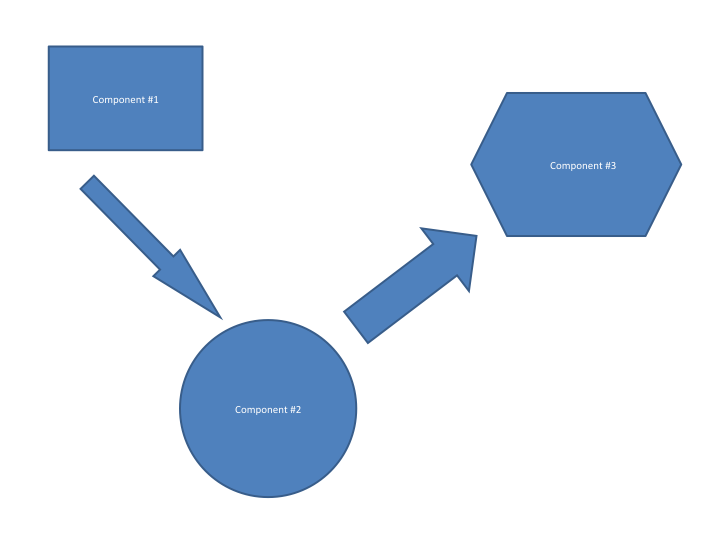
\includegraphics[width=0.75\textwidth]{./diagram}
\end{center}
\caption{A sample figure .... System Diagram \label{systemdiagram}}
\end{figure}

\section{Technologies Overview}
This section should contain a list of specific technologies used to
develop the system.  The list should contain the name of the
technology, brief description, link to reference material for further
understanding, and briefly how/where/why it was used in the system.
See Table~\ref{somenumbers}.  This is a floating table environment.
\LaTeX\ will try to put it close to where it was typeset but will not
allow the table to be split.

\begin{table}[tbh]
\caption{A sample Table ... some numbers. \label{somenumbers}}
\begin{center}
\begin{tabular}{|r|l|}
  \hline
  7C0 & hexadecimal \\
  3700 & octal \\ \cline{2-2}
  11111000000 & binary \\
  \hline \hline
  1984 & decimal \\
  \hline
\end{tabular}
\end{center}
\end{table}

  %% All tracks
% !TEX root = DesignDocument.tex


\chapter{Project Overview}
This section provides an overview of project management and a brief overview of the phases of the project.



\section{Team Members and Roles}
Team members and assigned roles:
\begin{itemize}
\item \textbf{Steven Huerta} - Team Lead, Simulation, AI Landing
\item \textbf{Christopher Smith} - Simulation, AI Landing
\item \textbf{Jonathan Dixon} - Visual Homography Landing
\item \textbf{Julian Brackins} - Visual Homography Landing
\item \textbf{Dylan Geyer} - UAV Build, Visual Homography Landing
\end{itemize}

\noindent Role assignments:
\begin{itemize}
\item \textbf{UAV Build} - Responsible for the physical assembly of the hexrotor, including wiring and mounting of hardware on the UAV.
\item \textbf{Visual Homography Landing} - Responsible for the development of an algorithm to calculate the distance and direction to the center of the landing pad. 
\item \textbf{AI Landing} - Responsible for the development of a landing algorithm utilizing an AI approach such as a neural net.
\item \textbf{Simulation} - Responsible for the development of a test environment wherein a simulated hexrotor utilizes the developed landing algorithms to evaluate the fitness of the landing algorithm.  
\end{itemize}



\section{Project  Management Approach}
This project is managed through the Agile framework. The sprints are three weeks with a one week pause between for evaluation and plan adaptation before the next sprint. Sprints 1, 2, and 3 comprise Phase 1. Sprints 4, 5, and 6 comprise Phase 2. Requirements for the project were collected by interviewing the client to form a set of user stories. These user stories provide a backlog managed on Trello. The user stories for this project represent composition of several tasks. Tasks are factored from the user stories and assigned to team members as that task relates to the project. These task assignments and their progress are managed on Trello. Issues and troubleshooting is handled through email and team meetings. The team division of work is to limit the dependencies between team members, so that issues encountered by one team member does not impact the progress of other team members. Tasks are sometimes added, altered, or removed so as to reflect a better size-up of the backlog item.



%This section will provide an explanation of the basic approach to managing the 
%project.  Typically, this would detail how the project will be managed through 
%a given Agile methodology.  The sprint length (i.e. 2 weeks) and product backlog 
%ownership and location (ex. Trello) are examples of what will be discussed.  An 
%overview of the system used to track sprint tasks, bug or trouble tickets, and 
%user stories would be warranted. 


\section{Phase  Overview}
\normalsize{\textbf{Phase 1}}
\begin{itemize}
\item \textbf{O-1}: As an owner, I want the UAV to autonomously take-off from the landing pad.
\item \textbf{O-2}: As an owner, I want the UAV to autonomously navigate through a series of waypoints.
\end{itemize}

\vspace{3mm}
\noindent\normalsize{\textbf{Phase 2}}
\begin{itemize}
\item \textbf{U-1}: As a user, I want to communicate the waypoints to the UAV.
\item \textbf{O-3}: As an owner, I want the UAV to autonomously return to the location of the landing pad.
\item \textbf{O-4}: As an owner, I want the UAV to autonomously land on the landing pad without damaging the craft.
\item \textbf{O-5}: As an owner, I want the UAV to autonomously land on the landing pad with the correct orientation.
\end{itemize}

%If the system will be implemented in phases, describe those phases/sub-phases (design, 
%implementation, testing, delivery) and the various milestones in this section. 
% This section should also contain a correlation between the phases of development 
%and the associated versioning of the system, i.e. major version, minor version, 
%revision. 

\section{Terminology and Acronyms}
\begin{itemize}
\item FCU - Flight Control Unit
\item ROS - Robot Operating System
\item GCS - Ground Conrol Station
\item UAV - Unmanned Aerial Vehicle
\end{itemize}
%Provide a list of terms used in the document that warrant definition.  Consider 
%industry or domain specific terms and acronyms as well as system specific. 
   %% All tracks
%% !TEX root = SystemTemplate.tex
\chapter{User Stories, Backlog and Requirements}
\section{Overview}
%The overview should take the form of an executive summary.  Give the reader a feel 
%for the purpose of the document, what is contained in the document, and an idea 
%of the purpose for the system or product. 

% The userstories 
%are provided by the stakeholders.  You will create he backlogs and the requirements, and document here.  
%This chapter should contain 
%details about each of the requirements and how the requirements are or will be 
%satisfied in the design and implementation of the system.

%Below:   list, describe, and define the requirements in this chapter.  
%There could be any number of sub-sections to help provide the necessary level of 
%detail. 
This section details the requirements(defined by the user stories) that set the goals, and subsequent tasks, of the project. This document will provide a more detailed view of the user stories. Additionally, this document will describe the client and developers more thoroughly.\\




\subsection{Scope}
This section includes the client information, user stories, and requirements. \\

%What scope does this document cover?  This document would contain stakeholder information, 
%initial user stories, requirements, proof of concept results, and various research 
%task results. 



\subsection{Purpose of the System}
The purpose of this project is to provide a prototype of implementing autonomous navigation and landing on a UAV platform. This project is a proof of concept, concentrating on landing algorithm approaches that will provide minimal error in terms of distance and orientation when landing. Ultimately, this technology will be integrated into the larger project where the UAV is capable of launching from an Unmanned Ground Vehicle(UVG), navigate in mild weather conditions, return, and land to recharge.\\


\section{ Stakeholder Information}
The Math and Computer Science Department of South Dakota School of Mines and Technology, in addi-
tion to providing ABET certified education to students, conducts software-side robotics research including
autonomy, navigation, and computer vision. Dr. Pyeatt is representing the school as the project sponsor, advisor, and project owner.\\


\subsection{Customer or End User (Product Owner)}
Dr. Pyeatt, representing the school, has articulated the project requirements. The team has used these requirements to create user stories as a means to factor the project into work products that can be more easily tracked. Dr. Pyeatt will provide feedback, as the project owner, to the team.\\ 

\subsection{Management or Instructor (Scrum Master)}
Dr. Pyeatt, as previously mentioned, is also the team's advisor. Dr. Pyeatt will provide the team with experience and expertise to assist the team with project development. Dr. Pyeatt assistance also includes providing feedback on approaches taken by the team, as well as providing recommendations. Dr. Pyeatt regularly attends weekly meeting, and has provided very liberal access for consultation outside of meetings.\\


\subsection{Investors}
The South Dakota School of Mines and Technology are the sole investors in this project.\\

%Are there any?  Who?  What role will they play? 


\subsection{Developers --Testers}
All team members will serve as developers, designers, and testers. Team members will initially be divided up to concentrate in areas of the project that are required. As the project progresses and development needs change, team members will be reassigned to other project areas. Team member assignments are:
\begin{itemize}
\item \textbf{Christopher Smith:} Simulation, AI Landing
\item \textbf{Steven Huerta:} Simulation, AI Landing
\item \textbf{Dylan Geyer:} UAV Build
\item \textbf{Jonathan Dixon:} Visual Homography Landing
\end{itemize}
%Who?  Is there a defined project manager, developer, tester, designer, architect, 
%etc.? 
\noindent The team 

%\section{Business Need}
%Use this section to define what business need exist and how this software will 
%meet and/or exceed that business need.   

\section{Requirements and Design Constraints}
%Use this section to discuss what requirements exist that deal with meeting the 
%business need.  These requirements might equate to design constraints which can 
%take the form of system, network, and/or user constraints.  Examples:  Windows 
%Server only, iOS only, slow network constraints, or no offline, local storage capabilities. 
The requirements for this project are:
\begin{itemize}
\item Ability to communicate waypoints to UAV.
\item UAV can autonomously take-off.
\item UAV can autonomously navigate through waypoints.
\item UAV can autonomously navigate back to landing pad.
\item UAV can autonomously land safely and with the correct orientation.
\end{itemize}

The only client defined constraint on this project is funding. We have limited funds, around \$1,000, to complete this project. However, more funds may become available depending on need and funding sources. Otherwise, this project does not have hard constraints set by the client, but rather are informed as a consequence of our design decisions.\\

\subsection{System  Requirements}
%What are they?  How will they impact the potential design?  Are there alternatives? 
The Pixhawk was selected as the flight controller for this project because of its built-in autonomy and open-source communication protocol, Mavlink, that will allow the team to use for message passing. \\

The ODroid was selected as the single board processor because of its processing power. The team will be running a ROS environment on Ubuntu 14.04. This eliminated a great number of boards from being candidates. The ODroid XU4 provides the power needed to run the environment without greatly impacting our project budget.\\ 

\subsection{Network Requirements}
%What are they? 
There are no network requirements for this project in regards to implementation.\\

\subsection{Development Environment Requirements}
%What are they?  Is the system supposed to be cross-platform? 
Development environment is Ubuntu 14.04. This is required because of our use of ROS. ROS distros Indigo/Jade require Ubuntu 14.04. The system will not be further developed to be cross-platform. As the purpose of this project is to provide a proof of concept, and there is not reliable Windows or Mac support for ROS, it would not be a responsible or worthwhile effort in producing cross-platform compatibility.\\

\subsection{Project  Management Methodology}
%The stakeholders might restrict how the project implementation will be managed. 
% There may be constraints on when design meetings will take place.  There might 
%be restrictions on how often progress reports need to be provided and to whom. 
% 
%\begin{itemize}
%\item What system will be used to keep track of the backlogs and sprint status?
%\item Will all parties have access to the Sprint and Product Backlogs?
%\item How many Sprints will encompass this particular project?
%\item How long are the Sprint Cycles?
%\item Are there restrictions on source control? 
%\end{itemize}

The team has elected to use Trello to keep track of backlogs and tasks. All team members have access to the trello web application. The Trello board is populated with a backlog representing the user stories. Each of these user stories will factor into a series of tasks that will be assigned at the beginning of each sprint.\\

This project will encompass a total of six sprints. Each sprint will span three weeks. Each semester will correspond with a phase, made up of three sprints. There will typically be a period of a week between each sprint, where a sprint report and prototypes will be made available for review.\\

The code and documentation for the project is maintained on github within a project repository. All team members, sponsor/advisor, and course instructor will have access to the repository. The agreed upon use of the repository is for team members to branch the repo to make changes as they are working on their functional area. When that team member is ready to integrate that branch back into the master, the team will conduct a code review. Each team member must be able to provide feedback before a merge can occur. The exception to this is documentation. Documentation may be merged as needed, so long as the team member has taken appropriate steps to ensure that the documentation is still in a function state after merging.\\

\section{User Stories}

\subsection{User Story \#1}
\textbf{User-1:} As a user, I want to communicate the waypoints to the UAV.

\subsubsection{User Story \#1 Breakdown}
The user will require some means of supplying waypoints and other mission parameters to the UAV. The team needs to explore possible approaches, as well as look at last year's attempt. \\
%Does the first user story need some division into smaller, consumable parts by 
%the reader?  This does not need to go to the level of actual task definition and 
%may not be required. 

\subsection{User Story \#2} 
\textbf{Owner-1:} As an owner, I want the UAV to autonomously take-off from the landing pad.

\subsubsection{User Story \#2 Breakdown}
The UAV will need to operate autonomously for the duration of the demonstration, to include take-off. The team will need to explore possible approaches, and refer to last year's attempt if possible. After some research, the team will need to implement this functionality. The team understands that this functionality will be gained through the use of the autonomy supplied with the flight controller, however the team needs to interface with the flight controller to enable that autonomy. \\

\subsection{User Story \#3} 
\textbf{Owner-2:} As an owner, I want the UAV to autonomously navigate through a series of waypoints.

\subsubsection{User Story \#3 Breakdown}
The UAV will need to be able to navigate through a series of waypoints defined ahead of time by the user. The team will need to explore possible approaches and refer to last year's attempt. The team will then need to implement this functionality. The team understands that this functionality is supplied with the flight controller. However, the team will still need to find a way to enable this functionality.\\

\subsection{User Story \#4} 
\textbf{Owner-3:} As an owner, I want the UAV to autonomously return to the location of the landing pad.

\subsubsection{User Story \#4 Breakdown}
The UAV will need to return the landing pad. Naively, this will occur after visiting the waypoints, however, there are other conditions that may necessitate the need to return to the landing pad such as finding the object of interest or running low on power. The team plans to address the first case (return after visiting all waypoints). Extension to this item may be addressed if the team completes the project with sufficient time remaining.\\ 


\subsection{User Story \#5} 
\textbf{Owner-4:} As an owner, I want the UAV to autonomously land on the landing pad without damaging the
craft

\subsubsection{User Story \#5 Breakdown}
The UAV will need to land on the landing pad with $\pm$.1m distance error. The team will explore visual homography and AI approaches. Each approach will have the goal of moving the UAV to the landing pad.\\ 


\subsection{User Story \#6} 
\textbf{Owner-5:} As an owner, I want the UAV to autonomously land on the landing pad with the correct orienta-
tion

\subsubsection{User Story \#6 Breakdown}
Building from the previous user story, the UAV will need to land with the correct orientation. Each of the previously mentioned algorithms will require that the UAV lands with $\pm$15$^{\circ}$ of correct orientation. However, the final project may see the fusion of different approaches to achieve the desired result. \\


%\section{Research or Proof of Concept Results}
%This section is reserved for the discussion centered on any research that needed 
%to take place before full system design.  The research efforts may have led to 
%the need to actually provide a proof of concept for approval by the stakeholders. 
%The proof of concept might even go to the extent of a user interface design or 
%mockups. 


%\section{Supporting Material}
%This document might contain references or supporting material which should be documented 
%and discussed  either here if appropriate or more often in the appendices at the end.  This material may have been provided by the %stakeholders  
%or it may be material garnered from research tasks.

  %% Not research track
% !TEX root = SystemTemplate.tex

\chapter{Design  and Implementation}
This section is used to describe the design details for each of the major components in the system. The autonomous systems of teh UAV can be broken into individual components and the following sections will be divided by such. The first section will cover our simulation environment, the second will cover the autonomous takeoff and waypoint navigation, the third section will discuss our two autonomous landing approaches, and finally the fourth section will cover the UAV.      

\section{Simulation Environment}
\subsection{Technologies  Used}
The simulation environment will be implemented using Gazebo as the actual environment itself and will use ROS so we can use the message passing services to communicate with different modules of code that will be written. This environment will handle all testing so nothing is tested on the physical UAV until it is verified working in a simulated environment that utilizes a pixhawk.
\subsection{Component  Overview}
\begin{itemize}
  \item Ubuntu 14.04 LTS
  \item Gazebo
  \item Mavlink
  \item python
  \item c++
  \item R.O.S.
  \item Mavros (Ros wrapper around Mavlink)
\end{itemize}
\subsection{Phase Overview}
The simulation environment is still a work in progress on setting up communication with a simulated pixhawk with software in the loop (SITL), however as soon as the pixhawk is received hardware in the loop (HITL) will be attempted because of issues simulating the device. Issues as of now are loading a waypoint file and sending commands. A file checksum appears to be invalid for the waypoint file and a invalid flight controller unit is returned after sending commands to the simulated pixhawk with the mavros cmd node.
\subsection{Design Details}
Currently the Design for the simulation is relying on outside sources for installing the environment and setting up packages. These details are discussed in the Prototype section within sprint report \#3.


\section{Autonomous Takeoff and Waypoint Navigation} 
\subsection{Technologies  Used}
The autonomous takeoff and waypoint navigation system is separate from the simulation environment and landing approaches because these will be contained in a mission that will be uploaded into the pixhawk. There will be a waypoint publisher (wpt\_pub) node that will receive input from a user and create a mission file out of that input. Another module within the node will start publishing waypoints to the node so that it nodes what path to take what to do using mavros messages.
\subsection{Component  Overview}
wpt\_pub dependencies:
\begin{itemize}
  \item Ubuntu 14.04 LTS
  \item python
  \item c++
  \item R.O.S.
  \item Mavros
  \item Mavros msgs
\end{itemize}
\subsection{Phase Overview}
The wpt\_pub node can currently publish mavros messages that contain take off, land, and arm commands successfully, however the simulated pixhawk reports back that it is an invalid flight controller unit most times. It does receive waypoints successfully through mavros messages.
\subsection{Design Details}
\lstinputlisting[language=C++]{code/wpt_pub.hpp}
\lstinputlisting[language=C++]{code/wpt_pub.cpp}
\lstinputlisting[language=C++]{code/wpt_pub_node.cpp}

\section{Landing Approaches}
\subsection{Visual Homography}
One of the approaches we will be using for the task of landing the UAV will be using visual homography. The basic goal here is to take an image that will contain the landing pad, and, based on the how the target looks on the pad, determine range to pad, orientation with respect to the pad, and the angle above the horizon with respect to the pad. This information will then be used to determine how to actually fly the UAV so that it will be able to safely land on the pad.
\subsubsection{Technologies  Used}
In order to accomplish this, we will use a number of tools. First and foremost, we will be using OpenCV as our image recognition library. OpenCV is a powerful open-source toolkit that will be able to handle any image processing that we need to do. The algorithm will be developed in Python, as this provides an easy-to-understand syntax, and will be able to deliver the performance that we need.
\subsubsection{Component  Overview}
\begin{itemize}
	\item Ubuntu 14.04 LTS
	\item Python
	\item OpenCV
\end{itemize}
\subsubsection{Phase Overview}
The algorithm is still a work in progress, but steps have been made. We have been able to compile and run last year's code, and have a working blob detection system up and running. This system is able to detect a pad with three colored circles by looking for the colors of the circles. The circles are red, green, and blue. It is then able to calculate the distance to the target, since it knows what size the target should be. This should be very helpful moving forward, as we are able to find the pad. In the coming sprints, we will attempt to move toward a pad that has four circles, as we believe this will give us more information to use for our homography computations.
\subsubsection{Design Details}
In the following image, you can see results from last year's code running and detecting the colored circles on a large target with three circles.

\begin{center} 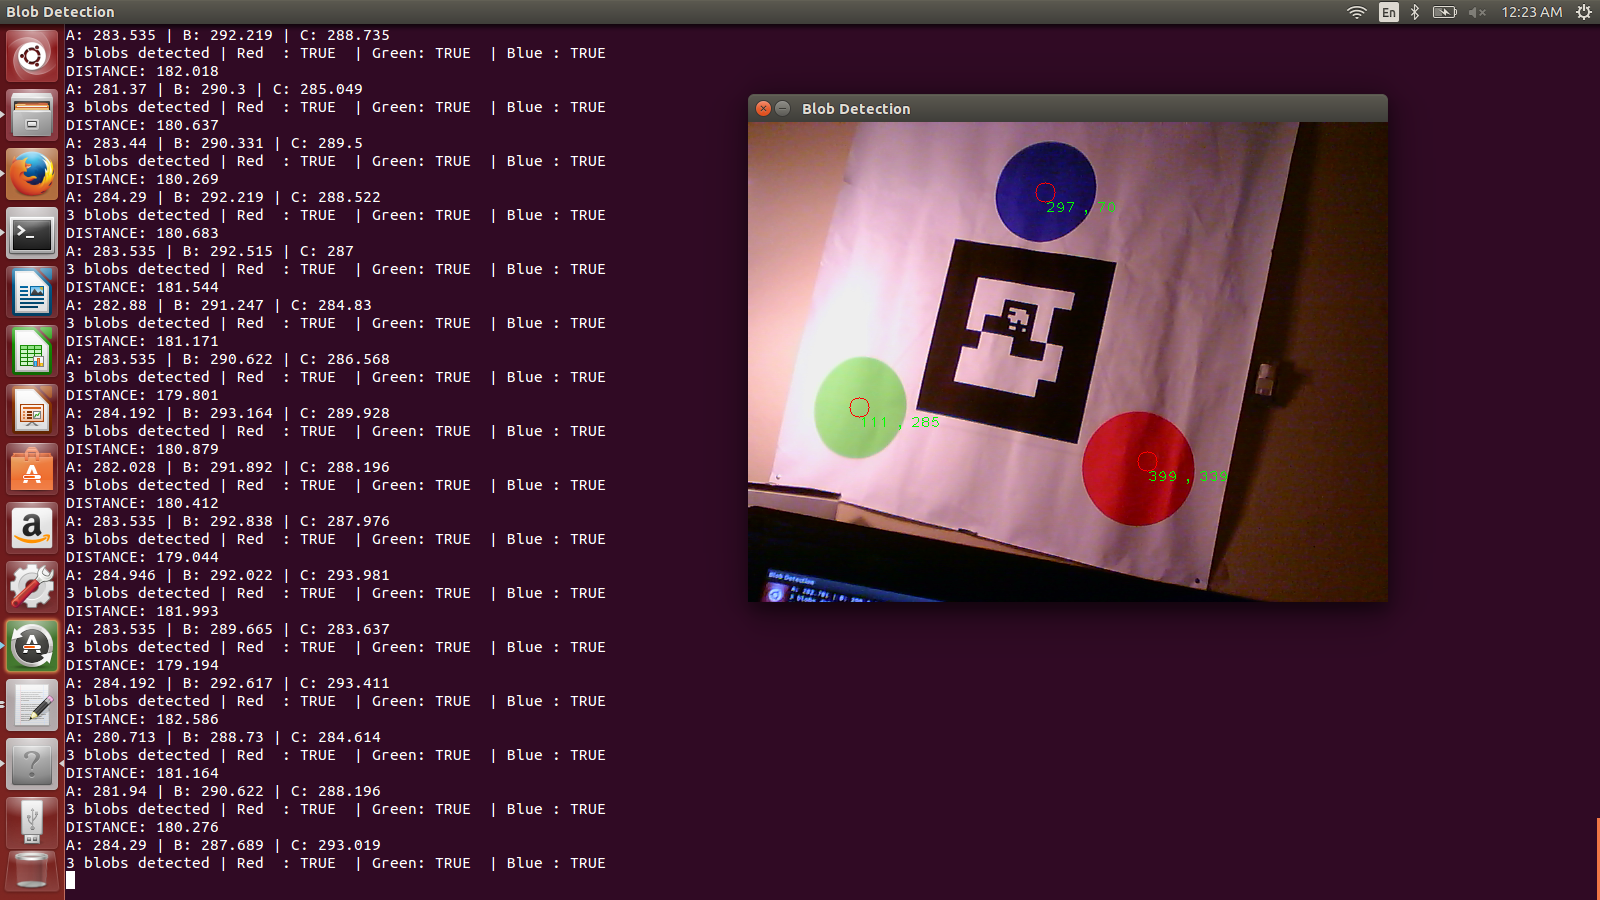
\includegraphics[width=.5\textwidth]{coolpic.png} \end{center}

It may be hard to notice, but the text that is currently being displayed in the terminal window shows that there are three blobs detected, exactly one for each color. It is also displaying the range to target, which is correct as far as we can tell.

The next image is what we are going to attempt to use for the next target. It has four colored circles, so we should be able to compute homography more accurately.

\begin{center} 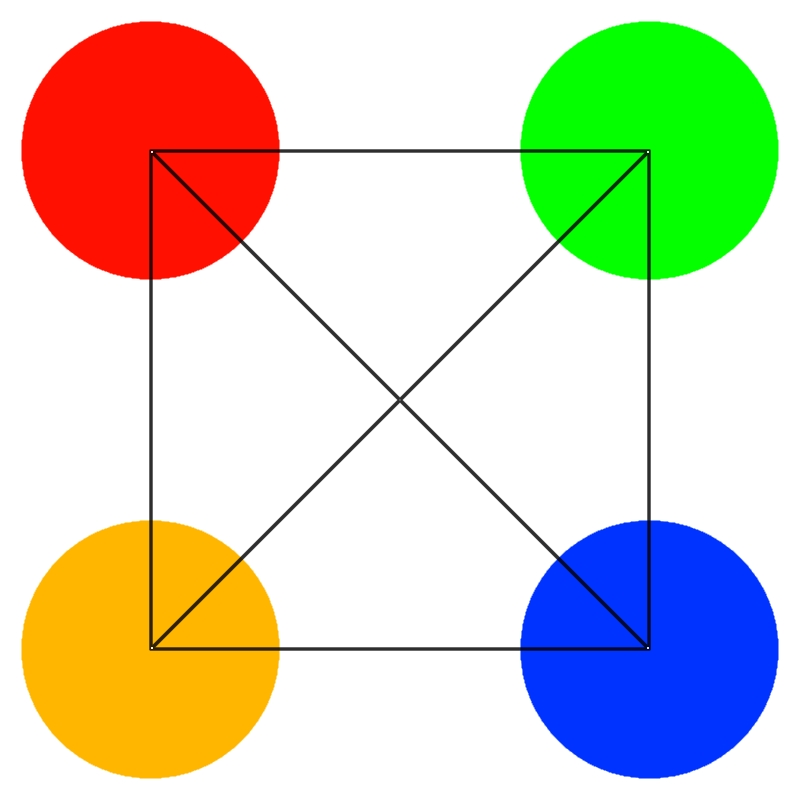
\includegraphics[width=.35\textwidth]{landing_guide_small_x.jpg} \end{center}

The final image is just another possible method that we have briefly explored where instead of blob detection we use hough transforms to detect only circles in the images. We have seen papers where others have had successes using targets consisting of concentric circles, so we think that we may be able to have some amount of success with this, in the event that the above methods don't end up panning out.

\begin{center} 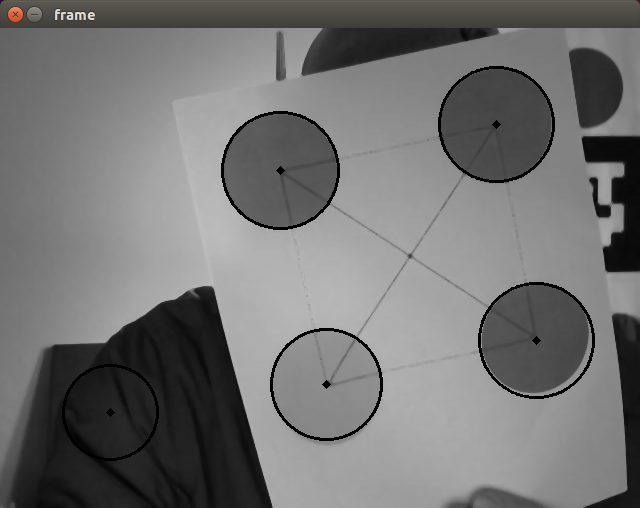
\includegraphics[width=.5\textwidth]{circles.png} \end{center}

\subsection{Reinforcement Learning}
\subsubsection{Technologies  Used}
\subsubsection{Component  Overview}
\subsubsection{Phase Overview}
\subsubsection{Design Details}

\section{UAV Build}
This section details the physical building of the UAV that will be used in autonomous landing.
\subsection{Technologies  Used}
The technologies that we currently have are listed below and include the controllers required for autonomous flight.
\begin{itemize}
	\item Turnigy Talong V1.0 Hexcopter
	\item 6x DC Motors
	\item 6x Electronic Speed Controllers
	\item 3DR Pixhawk
	\item Odroid-XU4
\end{itemize}
\subsection{Phase Overview}
We are currently in the first phase of UAV construction. In this phase we have completed the construction of the \textbf{Turnigy Talong V1.0 Hexcopter} frame, and mounting all of the DC motors and electronic speed controllers.
\subsection{Design Details}
Current documentation on the build progress made in Sprint 3 is shown below in our BuildProcess.pdf document.
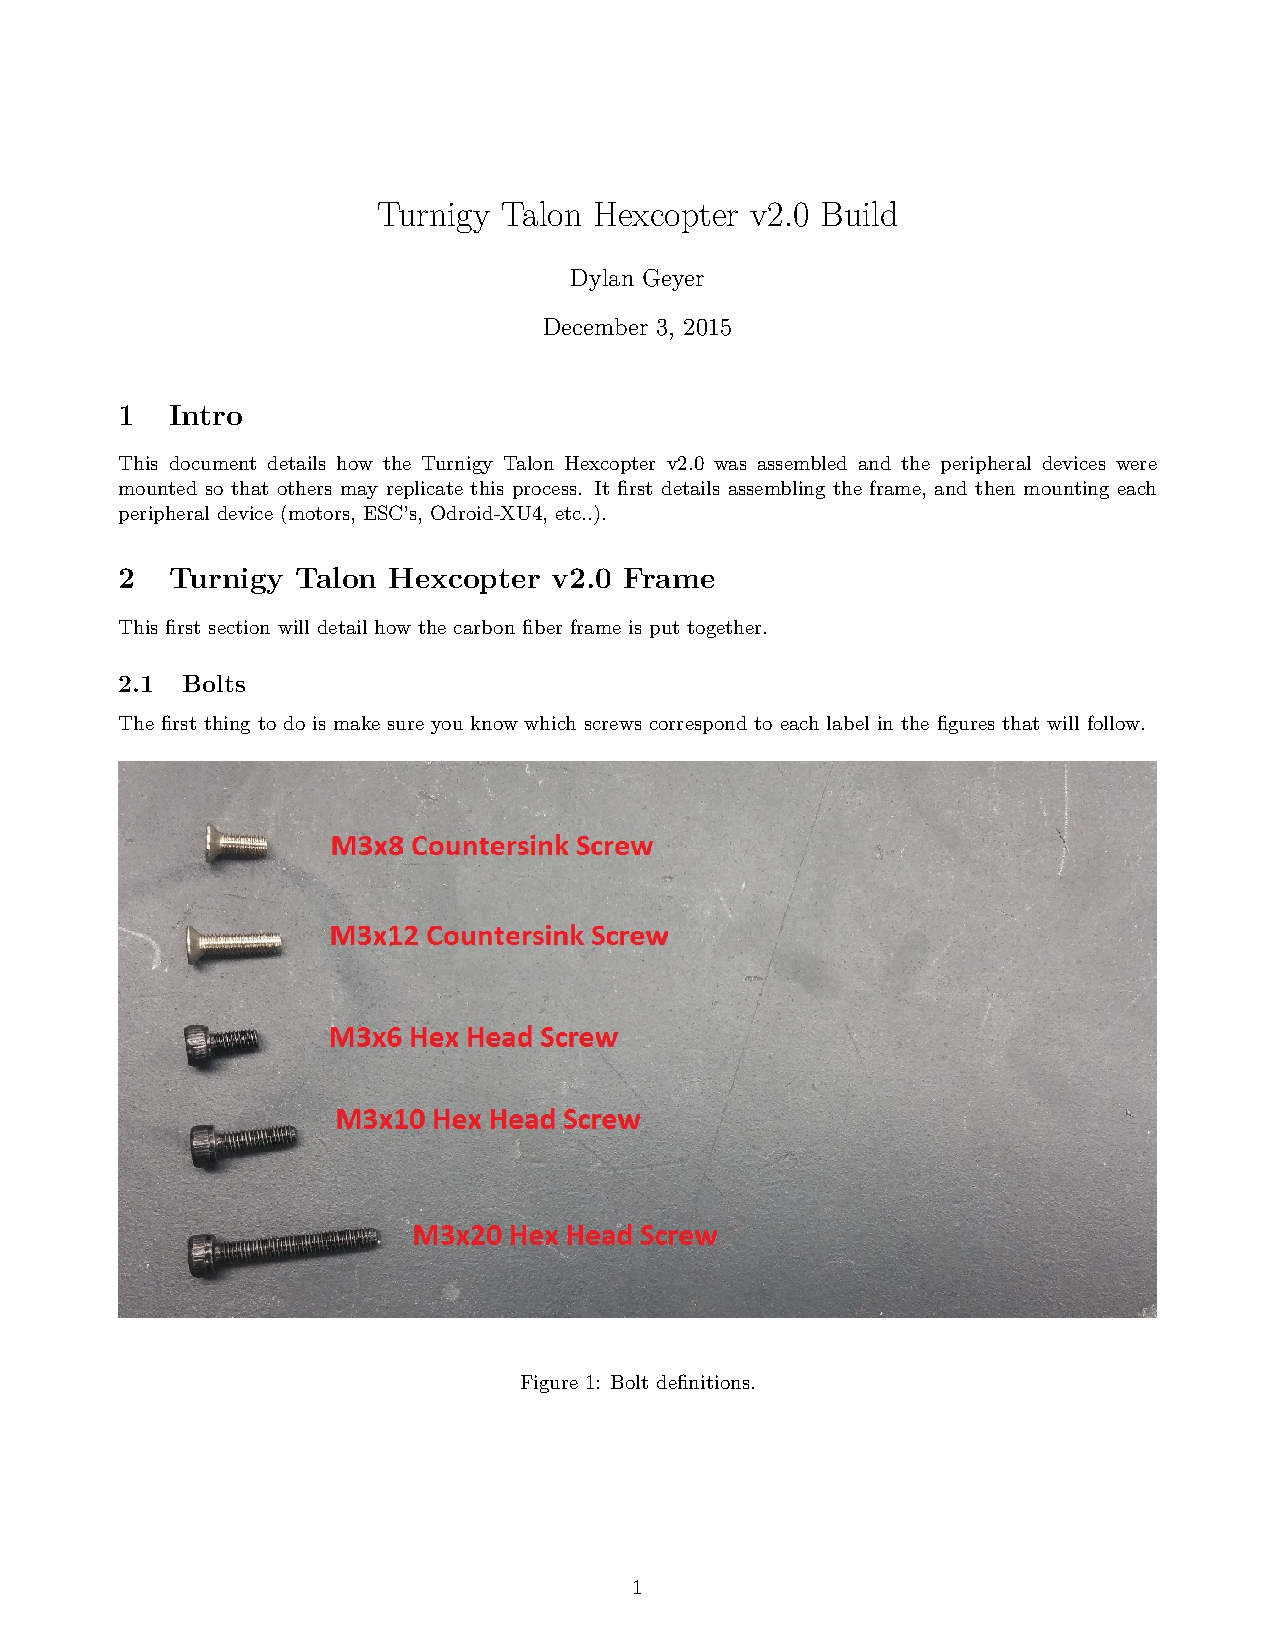
\includepdf[pages={1,2,3,4,5}]{../Prototypes/Sprint_3/BuildProcedure/BuildProcess.pdf}


%\begin{algorithm} [tbh]                     % enter the algorithm environment
%\caption{Calculate $y = x^n$}          % give the algorithm a caption
%\label{alg1}                           % and a label for \ref{} commands later in the document
%\begin{algorithmic}                    % enter the algorithmic environment
%    \REQUIRE $n \geq 0 \vee x \neq 0$
%    \ENSURE $y = x^n$
%    \STATE $y \Leftarrow 1$
%    \IF{$n < 0$}
%        \STATE $X \Leftarrow 1 / x$
%        \STATE $N \Leftarrow -n$
%    \ELSE
%        \STATE $X \Leftarrow x$
%        \STATE $N \Leftarrow n$
%    \ENDIF
%    \WHILE{$N \neq 0$}
%        \IF{$N$ is even}
%            \STATE $X \Leftarrow X \times X$
%            \STATE $N \Leftarrow N / 2$
%        \ELSE[$N$ is odd]
%            \STATE $y \Leftarrow y \times X$
%            \STATE $N \Leftarrow N - 1$
%        \ENDIF
%    \ENDWHILE
%\end{algorithmic}
%\end{algorithm} 
 
%\begin{lstlisting}
%#include <stdio.h>
%#define N 10
%/* Block
% * comment */
% 
%int main()
%{
%    int i;
% 
%    // Line comment.
%    puts("Hello world!");
% 
%    for (i = 0; i < N; i++)
%    {
%        puts("LaTeX is also great for programmers!");
%    }
% 
%    return 0;
%}
%\end{lstlisting}
%This code listing is not floating or automatically numbered.  If you want auto-numbering, but it in the algorithm environment (not algorithmic however) shown above.
  %% All tracks
% !TEX root = SystemTemplate.tex

\chapter{System  and Unit Testing}

This section describes the approach taken with regard to system and unit testing. 

\section{Overview}
Provides a brief overview of the testing approach, testing frameworks, and general 
how testing is/will be done to provide a measure of success for the system. 



\section{Dependencies}
Describe the basic dependencies which should include unit testing frameworks and 
reference material. 


\section{Test Setup and Execution}
Describe how test cases were developed, setup, and executed.  This section can 
be extremely involved if a complete list of test cases was warranted for the system. 

  %% All tracks
% !TEX root = UAV_Landing_Pad.tex
\chapter{Development Environment}
The basic purpose for this section is to give a developer all of the necessary 
information to setup their development environment to run, test, and/or develop. 


%\section{Development IDE and Tools}
%Describe which IDE and provide links to installs and/or reference material. 

\section{Source  Control}

The source code for our project is located on a private SVN repository provided by the Mathematics and Computer Science department at the South Dakota School of Mines and Technology. The repository is located at \url{http://dev.mcs.sdsmt.edu/repos/srdesign1415/robots/trunk/landingpad/}.

All of the code designed specifically to be put onto the UAV and UGV are located in the Build Directory, which is broken up into Build/UAV and Build/UGV environments. The Build/Environment directory is used for components that are present in both the UAV and the UGV.

%\section{Dependencies}
%Describe all dependencies associated with developing the system. 
%
%\section{Build  Environment}
%How are the packages built?  Are there build scripts? 

\section{Development Machine Setup}
An extensive list of walkthroughs for installing all major components of this project are outlined in the Appendix. Please refer to Section~\ref{walkthroughs} for more information on how to build each component for the development setup.
 %% All tracks
%% !TEX root = UAV_Landing_Pad.tex

\chapter{Release -- Setup -- Deployment}
This section should contain any specific subsection regarding specifics in releasing, 
setup, and/or deployment of the system. 


\section{Deployment Information and Dependencies}
Are there dependencies that are not embedded into the system install? 



\section{Setup Information}
How is a setup/install built? 



\section{System  Versioning Information}
How is the system versioned? 
  %% Normally not research track
% !TEX root = DesignDocument.tex

\chapter{User Documentation}

This chapter will cover the usage instructions and how to install the software required to get the UAV up an running with a Pixhawk flight controller and a odroid xu4 companion computer. The User Guide section will cover how to run all the software installed during the Installation Guide. The Programmer Manual section will cover where to get up to speed with programming in ROS as well as details regarding the flight controller code that was used to demonstrate offboard control.

%% \newpage  %%  if needed ...
\section{Installation Guide}
The following two sections will go through the set up of a laptop or desktop as a workstation and the odroid that will be attached to the UAV.
\subsection{Setting Up a Workstation}
To set up the workstation the first thing that is required is a computer with \href{http://www.ubuntu.com/download/desktop}{Ubuntu} 14.04 Long Term Support(LTS) installed as the operating system. 
\subsubsection{Dependencies}
Once a Ubuntu machine is acquired make sure git and cmake are installed by running the following commands: 
\begin{lstlisting}[language=bash]
$ sudo apt-get install git
$ sudo apt-get install cmake
\end{lstlisting}
Then create the following two directories:
\begin{lstlisting}[language=bash]
$ mkdir -p catkin_ws/src cmake_ws
\end{lstlisting}
These directories will be used to manage the libraries and software required by the UAV. The cmake\_ws will contain the source of the libraries required by a semi-direct monocular visual odometry pipeline package in ROS also known as SVO. The catkin\_ws directory will contain the source for SVO and other packages that will be written and downloaded for the UAV. Before any of the ROS packages can be installed the dependencies for SVO will need to be installed. \\
\\
The following commands will install Sophus which is required by SVO:
\begin{lstlisting}[language=bash]
$ cd cmake_ws
$ git clone https://github.com/strasdat/Sophus.git
$ cd Sophus
$ git checkout a621ff
$ mkdir build
$ cd build
$ cmake ..
$ make
\end{lstlisting}
The following commands will install Fast detector which is used by SVO to detect corners:
\begin{lstlisting}[language=bash]
$ cd cmake_ws
$ git clone https://github.com/uzh-rpg/fast.git
$ cd fast
$ mkdir build
$ cd build
$ cmake ..
$ make
\end{lstlisting}
Once Sophus and Fast are installed the ROS packages can start to be installed to the system.
\subsubsection{ROS}
To install ROS refer to \url{http://wiki.ros.org/indigo/Installation/Ubuntu}. It will always have the most up to date installation instructions for installing ROS indigo onto Ubuntu. Everything has successfully worked under both indigo and jade versions of ROS. If ROS jade has reached EOL then indigo should be used. The commands and links are given with ros-indigo instead of ros-jade for this purpose.\\
\\ 
To install mavros, ar-track-alvar, and the camera driver the following commands needs to be executed:
\begin{lstlisting}[language=bash]
$ sudo apt-get install ros-indigo-mavros*
$ sudo apt-get install ros-indigo-ar-track alvar
$ sudo apt-get install ros-indigo-pointgrey-camera-driver
\end{lstlisting}
In order to install ROS packages the catkin workspace will have to be initialized so that ROS libraries can be found for ROS packages that are written by a user or to compile source code. \\
\\
To initialize the catkin workspace execute the following:
\begin{lstlisting}[language=bash]
$ cd catkin_ws/src
$ catkin_init_workspace
$ cd ..
$ catkin_make
$ source devel/setup.bash
\end{lstlisting}
The source command above can be added to the .bashrc file in the home directory so the workspace doesn't have to be explicitly sourced. This will allow usage of packages compiled in this directory without having to remember to source it. \\
\\
Before SVO can be installed a ROS dependency vikit will need to be downloaded into the workspace alongside SVO.
\begin{lstlisting}[language=bash]
$ cd catkin_ws/src
$ git clone https://github.com/uzh-rpg/rpg_vikit.git
$ git clone https://github.com/uzh-rpg/rpg_svo.git
$ cd ..
$ catkin_make
\end{lstlisting}
Once all the previous software is set up, a couple of items need to be moved to specific directories on the system. The flight controller directory in the landingpad repository needs to be moved into the catkin/src directory that was used for SVO. Once that is done catkin\_make the directory again like above. Also the udev rules in the udev directory in the repository need to be moved to /etc/udev/rules.d/. The following commands will do the above, just replace directories with how it is set up on the system. This all assumes everything is in the home directory of the user. 
\begin{lstlisting}[language=bash]
$ cd
$ git clone https://github.com/SDSMT-CSC464-F15/landingpad
$ cd landingpad
$ cp -r flight_controller ../catkin_ws/src
$ cp udev/* /etc/udev/rules.d/
$ cd ../catkin_ws
$ catkin_make
$ source /devel/setup.bash
\end{lstlisting}
After all the steps are completed, the system is now ready for use and the user can run through the usage documentation on how to run everything that has just been installed. The next section will cover the instructions for the odroid.

\subsection{Setting Up the Odroid}
To set up the odroid that will be attached to the UAV the instructions for burning an image can be found here \url{http://odroid.com/dokuwiki/doku.php?id=en:odroid_flashing_tools}. The image that is required is the same as the odroid xu3 found at \url{http://odroid.com/dokuwiki/doku.php?id=en:xu3_release_linux_ubuntu}. It will be less demanding on the odroid if the sever version of the xu3 is used instead a desktop variant. Also space will be saved since a user interface is not necessary to run the commands on the odroid.\\
\\
Once the odroid is booting properly connect it to a monitor or ssh into it through the network to complete the rest of the installation. Before installing anything run the following command in the console:
\begin{lstlisting}[language=bash]
$ export ARM_ARCHITECTURE=True
\end{lstlisting}
After the above command is run the instructions for creating the directories and compiling the cmake libraries will work just like the workstation. However, the link above for the ROS directions is for a laptop or desktop computer that will be running ROS. The directions change since the odroid is a single board computer that uses the ARM architecture. The instructions for this can be found on the ROS website at \url{http://wiki.ros.org/indigo/Installation/UbuntuARM}. The rest of the instructions in the workstation section can be followed once ROS is installed on the odroid. Only the flight controller directory and udev rules from the repository should go on the odroid so space is not taken up by documents such as the design document and other miscellaneous items.

%% \newpage  %%  if needed ...
\section{User Guide}
Once all the software is installed successfully everything can start to be tested and ran. Make sure the ROS install is sourced correctly as well as the catkin workspace that was created during the installation section.\\
\\
This Section will cover how to run the flight controller code that was used to demonstrate offboard control, Ar-Track-Alvar for the tracking of ar tags, and the visual odometry package SVO for position estimates.\\
\\
The tools that will be used to run these packages and associated ros nodes will be roslaunch, and rosrun. More detail is given the the programmers manual on usage with ROS specific commands. 
\subsection{Flight Controller}
The flight controller node is a simple python node that can control the UAV by sending vectors of direction to go where the origin is where the UAV was turned on. The node is currently is not part of a launch file so switching between terminals will be necessary to get this running.
\subsection{Ar-Track-Alvar}
\subsection{SVO}

\section{Programmer Manual}
There are two main software packages used in this project ROS and mavlink. The robot operating system (ROS) is an open-source, meta-operating system for a robot, and Mavlink is the library used to interface with the Pixhawk flight controller.
\subsection{ROS}
ROS was the main the tool used in getting all the software to work together as well as many of the libraries in ROS are required to get different nodes to communicate with each other. The framework of ROS is complicated, but at its core it is an easy way to get different modules of code to communicate to each other. It has software built in that will allow a user to visualize the data that is getting streamed across the ROS network known as ROS topics.\\
\\
ROS provides wrappers for interfacing with low level libraries such as Mavlink. This allows data to get streamed accros ROS topics for the user to see what GPS location the flight controller and other useful information. The visulization tools such as Rviz allow a user to see pose information between a camera and ar tag for example as well as the map.\\
\\
\subsubsection{Core ROS Tools}
This section will cover the tools used specifically in the user guide. More information can be found at the ROS wiki regarding other tools or more in depth explanations.\\
\\
Roscore is a collection of nodes and programs that are pre-requisites of a ROS-based system. You must have a roscore running in order for ROS nodes to communicate. It is rand by using the roscore command.
\begin{lstlisting}[language=bash]
$ roscore
\end{lstlisting}
Rosrun allows you to run an executable in an arbitrary package from anywhere without having to give its full path.
\begin{lstlisting}[language=bash]
$ rosrun package executable
\end{lstlisting}
Roslaunch is a tool for easily launching multiple ROS nodes locally and remotely via SSH, as well as setting parameters on the Parameter Server. roslaunch can be run by executing the following commands.
\begin{lstlisting}[language=bash]
$ roslaunch package_name file.launch
\end{lstlisting}
Rostopic contains the rostopic command-line tool for displaying debug information about ROS Topics, including publishers, subscribers, publishing rate, and ROS Messages.
\begin{lstlisting}[language=bash]
$ rostopic list
$ rostopic echo topic_name
\end{lstlisting}
\subsection{Mavlink} %% All tracks
\documentclass[twoside]{book}

% Packages required by doxygen
\usepackage{calc}
\usepackage{doxygen}
\usepackage{graphicx}
\usepackage[utf8]{inputenc}
\usepackage{makeidx}
\usepackage{multicol}
\usepackage{multirow}
\usepackage{textcomp}
\usepackage[table]{xcolor}

% Font selection
\usepackage[T1]{fontenc}
\usepackage{mathptmx}
\usepackage[scaled=.90]{helvet}
\usepackage{courier}
\usepackage{amssymb}
\usepackage{sectsty}
\renewcommand{\familydefault}{\sfdefault}
\allsectionsfont{%
  \fontseries{bc}\selectfont%
  \color{darkgray}%
}
\renewcommand{\DoxyLabelFont}{%
  \fontseries{bc}\selectfont%
  \color{darkgray}%
}

% Page & text layout
\usepackage{geometry}
\geometry{%
  a4paper,%
  top=2.5cm,%
  bottom=2.5cm,%
  left=2.5cm,%
  right=2.5cm%
}
\tolerance=750
\hfuzz=15pt
\hbadness=750
\setlength{\emergencystretch}{15pt}
\setlength{\parindent}{0cm}
\setlength{\parskip}{0.2cm}
\makeatletter
\renewcommand{\paragraph}{%
  \@startsection{paragraph}{4}{0ex}{-1.0ex}{1.0ex}{%
    \normalfont\normalsize\bfseries\SS@parafont%
  }%
}
\renewcommand{\subparagraph}{%
  \@startsection{subparagraph}{5}{0ex}{-1.0ex}{1.0ex}{%
    \normalfont\normalsize\bfseries\SS@subparafont%
  }%
}
\makeatother

% Headers & footers
\usepackage{fancyhdr}
\pagestyle{fancyplain}
\fancyhead[LE]{\fancyplain{}{\bfseries\thepage}}
\fancyhead[CE]{\fancyplain{}{}}
\fancyhead[RE]{\fancyplain{}{\bfseries\leftmark}}
\fancyhead[LO]{\fancyplain{}{\bfseries\rightmark}}
\fancyhead[CO]{\fancyplain{}{}}
\fancyhead[RO]{\fancyplain{}{\bfseries\thepage}}
\fancyfoot[LE]{\fancyplain{}{}}
\fancyfoot[CE]{\fancyplain{}{}}
\fancyfoot[RE]{\fancyplain{}{\bfseries\scriptsize Generated on Sun Feb 8 2015 13\-:11\-:37 for My Project by Doxygen }}
\fancyfoot[LO]{\fancyplain{}{\bfseries\scriptsize Generated on Sun Feb 8 2015 13\-:11\-:37 for My Project by Doxygen }}
\fancyfoot[CO]{\fancyplain{}{}}
\fancyfoot[RO]{\fancyplain{}{}}
\renewcommand{\footrulewidth}{0.4pt}
\renewcommand{\chaptermark}[1]{%
  \markboth{#1}{}%
}
\renewcommand{\sectionmark}[1]{%
  \markright{\thesection\ #1}%
}

% Indices & bibliography
\usepackage{natbib}
\usepackage[titles]{tocloft}
\setcounter{tocdepth}{3}
\setcounter{secnumdepth}{5}
\makeindex

% Hyperlinks (required, but should be loaded last)
\usepackage{ifpdf}
\ifpdf
  \usepackage[pdftex,pagebackref=true]{hyperref}
\else
  \usepackage[ps2pdf,pagebackref=true]{hyperref}
\fi
\hypersetup{%
  colorlinks=true,%
  linkcolor=blue,%
  citecolor=blue,%
  unicode%
}

% Custom commands
\newcommand{\clearemptydoublepage}{%
  \newpage{\pagestyle{empty}\cleardoublepage}%
}


%===== C O N T E N T S =====

\begin{document}

% Titlepage & ToC
\hypersetup{pageanchor=false}
\pagenumbering{roman}
\begin{titlepage}
\vspace*{7cm}
\begin{center}%
{\Large My Project }\\
\vspace*{1cm}
{\large Generated by Doxygen 1.8.6}\\
\vspace*{0.5cm}
{\small Sun Feb 8 2015 13:11:37}\\
\end{center}
\end{titlepage}
\clearemptydoublepage
\tableofcontents
\clearemptydoublepage
\pagenumbering{arabic}
\hypersetup{pageanchor=true}

%--- Begin generated contents ---
\chapter{R\-O\-S A\-P\-I}
\label{index}\hypertarget{index}{}\hypertarget{index_course_section}{}\section{C\-S\-C 465}\label{index_course_section}
\begin{DoxyAuthor}{Author}
Alex Wulff
\end{DoxyAuthor}
\begin{DoxyDate}{Date}
December 15, 2014
\end{DoxyDate}
\begin{DoxyParagraph}{Professor\-:}
Dr. Jeff Mc\-Gough
\end{DoxyParagraph}
\begin{DoxyParagraph}{Course\-:}
C\-S\-C 465 -\/ M001 -\/ Tues / Thurs -\/ 9\-:00am
\end{DoxyParagraph}
\begin{DoxyParagraph}{Location\-:}
Mc\-Laury -\/ 304
\end{DoxyParagraph}
\hypertarget{index_program_section}{}\section{Program Information}\label{index_program_section}
This A\-P\-I for R\-O\-S node communication is developed for ease of subscription for topics on custom nodes. This will assist in the completion of the U\-G\-V/ U\-A\-V project for which we were all indroctinated. This was heavily borrowed from \href{http://wiki.ros.org/ROS/Tutorials}{\tt http\-://wiki.\-ros.\-org/\-R\-O\-S/\-Tutorials}.\hypertarget{index_compile_section}{}\section{Compiling and Usage}\label{index_compile_section}
\begin{DoxyParagraph}{Compiling Instructions\-:}
(Linux) -\/ catkin\-\_\-make
\end{DoxyParagraph}
\begin{DoxyParagraph}{Usage\-:}
\begin{DoxyVerb}rosrun api Api
\end{DoxyVerb}

\end{DoxyParagraph}
\hypertarget{index_todo_bugs_modification_section}{}\section{Todo, Bugs, and Modifications}\label{index_todo_bugs_modification_section}
\begin{DoxyParagraph}{Modifications and Development Timeline\-:}
\begin{DoxyVerb}Date              Modification
----------------  --------------------------------------------------------------
* December 15, 2014 Thought about an API.
*
* January 1-14, 2015    Created archtype and initial documentation.
*
* January 22, 2015  Began cross access of topics.
*
* January 29, 2015  Was advised to subdivide the API into each topic set then
*                      rebuild the base.
*
* February 2-5, 2015   Rebuilt structure and started debugging.
*
* February 8, 2015  Finished base structure and added documentation.
*
\end{DoxyVerb}
 
\end{DoxyParagraph}

\chapter{Ros Package File}
\label{Package}
\hypertarget{Package}{}

\begin{DoxyVerbInclude}
\end{DoxyVerbInclude}
 
\chapter{C\-Make\-List File}
\label{CMakeList}
\hypertarget{CMakeList}{}

\begin{DoxyVerbInclude}
\end{DoxyVerbInclude}
 
\chapter{File Index}
\section{File List}
Here is a list of all documented files with brief descriptions\-:\begin{DoxyCompactList}
\item\contentsline{section}{\hyperlink{Api_8C}{Api.\-C} \\*S\-O\-U\-R\-C\-E -\/ main file }{\pageref{Api_8C}}{}
\item\contentsline{section}{\hyperlink{Camera_8C}{Camera.\-C} \\*S\-O\-U\-R\-C\-E -\/ camera file }{\pageref{Camera_8C}}{}
\item\contentsline{section}{\hyperlink{CV_8C}{C\-V.\-C} \\*S\-O\-U\-R\-C\-E -\/ cv file }{\pageref{CV_8C}}{}
\item\contentsline{section}{\hyperlink{GPS_8C}{G\-P\-S.\-C} \\*S\-O\-U\-R\-C\-E -\/ G\-P\-S file }{\pageref{GPS_8C}}{}
\item\contentsline{section}{\hyperlink{Motors_8C}{Motors.\-C} \\*S\-O\-U\-R\-C\-E -\/ motors file }{\pageref{Motors_8C}}{}
\item\contentsline{section}{\hyperlink{Sender_8C}{Sender.\-C} \\*S\-O\-U\-R\-C\-E -\/ sender file }{\pageref{Sender_8C}}{}
\item\contentsline{section}{\hyperlink{Sim_8C}{Sim.\-C} \\*S\-O\-U\-R\-C\-E -\/ sim file }{\pageref{Sim_8C}}{}
\end{DoxyCompactList}

\chapter{File Documentation}
\hypertarget{Api_8C}{\section{Api.\-C File Reference}
\label{Api_8C}\index{Api.\-C@{Api.\-C}}
}


S\-O\-U\-R\-C\-E -\/ main file.  


{\ttfamily \#include \char`\"{}ros/ros.\-h\char`\"{}}\\*
{\ttfamily \#include \char`\"{}std\-\_\-msgs/\-String.\-h\char`\"{}}\\*
{\ttfamily \#include $<$pthread.\-h$>$}\\*
\subsection*{Functions}
\begin{DoxyCompactItemize}
\item 
void \hyperlink{Api_8C_ae5c0c11b4a60030ee8df1a3ae0b6f758}{chatter\-Callback} (const std\-\_\-msgs\-::\-String\-::\-Const\-Ptr \&msg)
\item 
\hypertarget{Api_8C_a38ce59a361b9595b45f8f358340511cd}{void {\bfseries G\-P\-S\-Callback} (const std\-\_\-msgs\-::\-String\-::\-Const\-Ptr \&msg)}\label{Api_8C_a38ce59a361b9595b45f8f358340511cd}

\item 
\hypertarget{Api_8C_a454ca9b8bf0da57a526dc3d1ec67063d}{void {\bfseries Error\-Callback} (const std\-\_\-msgs\-::\-String\-::\-Const\-Ptr \&msg)}\label{Api_8C_a454ca9b8bf0da57a526dc3d1ec67063d}

\item 
\hypertarget{Api_8C_ada0ab9274cab357d9df4f464d272b3a8}{void {\bfseries Other\-Callback} (const std\-\_\-msgs\-::\-String\-::\-Const\-Ptr \&msg)}\label{Api_8C_ada0ab9274cab357d9df4f464d272b3a8}

\item 
\hypertarget{Api_8C_a519247b7260f3560e1c3b06e8b4341ac}{void {\bfseries Cam\-Callback} (const std\-\_\-msgs\-::\-String\-::\-Const\-Ptr \&msg)}\label{Api_8C_a519247b7260f3560e1c3b06e8b4341ac}

\item 
\hypertarget{Api_8C_a77009212af45d6269d56d92dbadba018}{void {\bfseries C\-V\-Callback} (const std\-\_\-msgs\-::\-String\-::\-Const\-Ptr \&msg)}\label{Api_8C_a77009212af45d6269d56d92dbadba018}

\item 
\hypertarget{Api_8C_aa12c949b461f4739e395d3a646a9717e}{void {\bfseries Motor\-Callback} (const std\-\_\-msgs\-::\-String\-::\-Const\-Ptr \&msg)}\label{Api_8C_aa12c949b461f4739e395d3a646a9717e}

\item 
\hypertarget{Api_8C_a4c83938eb3fd2048fc4ce4e0589b980c}{void {\bfseries Slam\-Callback} (const std\-\_\-msgs\-::\-String\-::\-Const\-Ptr \&msg)}\label{Api_8C_a4c83938eb3fd2048fc4ce4e0589b980c}

\item 
\hypertarget{Api_8C_a1185378573b23c509dc41b1376a81ab2}{void {\bfseries Sim\-Callback} (const std\-\_\-msgs\-::\-String\-::\-Const\-Ptr \&msg)}\label{Api_8C_a1185378573b23c509dc41b1376a81ab2}

\item 
int \hyperlink{Api_8C_a3c04138a5bfe5d72780bb7e82a18e627}{main} (int argc, char $\ast$$\ast$argv)
\end{DoxyCompactItemize}


\subsection{Detailed Description}
S\-O\-U\-R\-C\-E -\/ main file. 

\subsection{Function Documentation}
\hypertarget{Api_8C_ae5c0c11b4a60030ee8df1a3ae0b6f758}{\index{Api.\-C@{Api.\-C}!chatter\-Callback@{chatter\-Callback}}
\index{chatter\-Callback@{chatter\-Callback}!Api.C@{Api.\-C}}
\subsubsection[{chatter\-Callback}]{\setlength{\rightskip}{0pt plus 5cm}void chatter\-Callback (
\begin{DoxyParamCaption}
\item[{const std\-\_\-msgs\-::\-String\-::\-Const\-Ptr \&}]{msg}
\end{DoxyParamCaption}
)}}\label{Api_8C_ae5c0c11b4a60030ee8df1a3ae0b6f758}
This tutorial demonstrates simple receipt of messages over the R\-O\-S system. \hypertarget{Api_8C_a3c04138a5bfe5d72780bb7e82a18e627}{\index{Api.\-C@{Api.\-C}!main@{main}}
\index{main@{main}!Api.C@{Api.\-C}}
\subsubsection[{main}]{\setlength{\rightskip}{0pt plus 5cm}int main (
\begin{DoxyParamCaption}
\item[{int}]{argc, }
\item[{char $\ast$$\ast$}]{argv}
\end{DoxyParamCaption}
)}}\label{Api_8C_a3c04138a5bfe5d72780bb7e82a18e627}
The ros\-::init() function needs to see argc and argv so that it can perform any R\-O\-S arguments and name remapping that were provided at the command line. For programmatic remappings you can use a different version of init() which takes remappings directly, but for most command-\/line programs, passing argc and argv is the easiest way to do it. The third argument to init() is the name of the node.

You must call one of the versions of ros\-::init() before using any other part of the R\-O\-S system.

Node\-Handle is the main access point to communications with the R\-O\-S system. The first Node\-Handle constructed will fully initialize this node, and the last Node\-Handle destructed will close down the node.

The subscribe() call is how you tell R\-O\-S that you want to receive messages on a given topic. This invokes a call to the R\-O\-S master node, which keeps a registry of who is publishing and who is subscribing. Messages are passed to a callback function, here called chatter\-Callback. subscribe() returns a Subscriber object that you must hold on to until you want to unsubscribe. When all copies of the Subscriber object go out of scope, this callback will automatically be unsubscribed from this topic.

The second parameter to the subscribe() function is the size of the message queue. If messages are arriving faster than they are being processed, this is the number of messages that will be buffered up before beginning to throw away the oldest ones.

ros\-::spin() will enter a loop, pumping callbacks. With this version, all callbacks will be called from within this thread (the main one). ros\-::spin() will exit when Ctrl-\/\-C is pressed, or the node is shutdown by the master.
\hypertarget{Camera_8C}{\section{Camera.\-C File Reference}
\label{Camera_8C}\index{Camera.\-C@{Camera.\-C}}
}


S\-O\-U\-R\-C\-E -\/ camera file.  


{\ttfamily \#include \char`\"{}ros/ros.\-h\char`\"{}}\\*
{\ttfamily \#include \char`\"{}std\-\_\-msgs/\-String.\-h\char`\"{}}\\*
\subsection*{Functions}
\begin{DoxyCompactItemize}
\item 
\hypertarget{Camera_8C_a14253152440fb4c98ddeeb03c766a3c0}{void {\bfseries camera\-Callback} (const std\-\_\-msgs\-::\-String\-::\-Const\-Ptr \&msg)}\label{Camera_8C_a14253152440fb4c98ddeeb03c766a3c0}

\item 
\hypertarget{Camera_8C_a3c04138a5bfe5d72780bb7e82a18e627}{int {\bfseries main} (int argc, char $\ast$$\ast$argv)}\label{Camera_8C_a3c04138a5bfe5d72780bb7e82a18e627}

\end{DoxyCompactItemize}
\subsection*{Variables}
\begin{DoxyCompactItemize}
\item 
\hypertarget{Camera_8C_aec4c7a9801a00f27f39f6bd77aec69ca}{ros\-::\-Publisher {\bfseries cam\-Stream\-\_\-pub}}\label{Camera_8C_aec4c7a9801a00f27f39f6bd77aec69ca}

\end{DoxyCompactItemize}


\subsection{Detailed Description}
S\-O\-U\-R\-C\-E -\/ camera file. 
\hypertarget{CV_8C}{\section{C\-V.\-C File Reference}
\label{CV_8C}\index{C\-V.\-C@{C\-V.\-C}}
}


S\-O\-U\-R\-C\-E -\/ cv file.  


{\ttfamily \#include \char`\"{}ros/ros.\-h\char`\"{}}\\*
{\ttfamily \#include \char`\"{}std\-\_\-msgs/\-String.\-h\char`\"{}}\\*
\subsection*{Functions}
\begin{DoxyCompactItemize}
\item 
\hypertarget{CV_8C_a77009212af45d6269d56d92dbadba018}{void {\bfseries C\-V\-Callback} (const std\-\_\-msgs\-::\-String\-::\-Const\-Ptr \&msg)}\label{CV_8C_a77009212af45d6269d56d92dbadba018}

\item 
\hypertarget{CV_8C_a3c04138a5bfe5d72780bb7e82a18e627}{int {\bfseries main} (int argc, char $\ast$$\ast$argv)}\label{CV_8C_a3c04138a5bfe5d72780bb7e82a18e627}

\end{DoxyCompactItemize}
\subsection*{Variables}
\begin{DoxyCompactItemize}
\item 
\hypertarget{CV_8C_a85c99c78793120993218165ca0e4c3c4}{ros\-::\-Publisher {\bfseries C\-V\-Stream\-\_\-pub}}\label{CV_8C_a85c99c78793120993218165ca0e4c3c4}

\end{DoxyCompactItemize}


\subsection{Detailed Description}
S\-O\-U\-R\-C\-E -\/ cv file. 
\hypertarget{GPS_8C}{\section{G\-P\-S.\-C File Reference}
\label{GPS_8C}\index{G\-P\-S.\-C@{G\-P\-S.\-C}}
}


S\-O\-U\-R\-C\-E -\/ G\-P\-S file.  


{\ttfamily \#include \char`\"{}ros/ros.\-h\char`\"{}}\\*
{\ttfamily \#include \char`\"{}std\-\_\-msgs/\-String.\-h\char`\"{}}\\*
{\ttfamily \#include $<$sys/time.\-h$>$}\\*
\subsection*{Functions}
\begin{DoxyCompactItemize}
\item 
\hypertarget{GPS_8C_a479e2c182792f10b8967ab2a460b706c}{void {\bfseries gps\-Callback} (const std\-\_\-msgs\-::\-String\-::\-Const\-Ptr \&msg)}\label{GPS_8C_a479e2c182792f10b8967ab2a460b706c}

\item 
\hypertarget{GPS_8C_a3c04138a5bfe5d72780bb7e82a18e627}{int {\bfseries main} (int argc, char $\ast$$\ast$argv)}\label{GPS_8C_a3c04138a5bfe5d72780bb7e82a18e627}

\end{DoxyCompactItemize}
\subsection*{Variables}
\begin{DoxyCompactItemize}
\item 
\hypertarget{GPS_8C_a8748ba2164866b808be38475eb8345df}{ros\-::\-Publisher {\bfseries gps\-Stream\-\_\-pub}}\label{GPS_8C_a8748ba2164866b808be38475eb8345df}

\end{DoxyCompactItemize}


\subsection{Detailed Description}
S\-O\-U\-R\-C\-E -\/ G\-P\-S file. 
\hypertarget{Motors_8C}{\section{Motors.\-C File Reference}
\label{Motors_8C}\index{Motors.\-C@{Motors.\-C}}
}


S\-O\-U\-R\-C\-E -\/ motors file.  


{\ttfamily \#include \char`\"{}ros/ros.\-h\char`\"{}}\\*
{\ttfamily \#include \char`\"{}std\-\_\-msgs/\-String.\-h\char`\"{}}\\*
\subsection*{Functions}
\begin{DoxyCompactItemize}
\item 
\hypertarget{Motors_8C_a2c688cc695ddd0fe02f043502d2beae6}{void {\bfseries motor\-Callback} (const std\-\_\-msgs\-::\-String\-::\-Const\-Ptr \&msg)}\label{Motors_8C_a2c688cc695ddd0fe02f043502d2beae6}

\item 
\hypertarget{Motors_8C_a3c04138a5bfe5d72780bb7e82a18e627}{int {\bfseries main} (int argc, char $\ast$$\ast$argv)}\label{Motors_8C_a3c04138a5bfe5d72780bb7e82a18e627}

\end{DoxyCompactItemize}
\subsection*{Variables}
\begin{DoxyCompactItemize}
\item 
\hypertarget{Motors_8C_a513a68bcf99ae6280b951fd23006aa5e}{ros\-::\-Publisher {\bfseries motor\-Stream\-\_\-pub}}\label{Motors_8C_a513a68bcf99ae6280b951fd23006aa5e}

\end{DoxyCompactItemize}


\subsection{Detailed Description}
S\-O\-U\-R\-C\-E -\/ motors file. 
\hypertarget{Sender_8C}{\section{Sender.\-C File Reference}
\label{Sender_8C}\index{Sender.\-C@{Sender.\-C}}
}


S\-O\-U\-R\-C\-E -\/ sender file.  


{\ttfamily \#include \char`\"{}ros/ros.\-h\char`\"{}}\\*
{\ttfamily \#include \char`\"{}std\-\_\-msgs/\-String.\-h\char`\"{}}\\*
{\ttfamily \#include $<$sstream$>$}\\*
\subsection*{Functions}
\begin{DoxyCompactItemize}
\item 
int \hyperlink{Sender_8C_a3c04138a5bfe5d72780bb7e82a18e627}{main} (int argc, char $\ast$$\ast$argv)
\end{DoxyCompactItemize}


\subsection{Detailed Description}
S\-O\-U\-R\-C\-E -\/ sender file. 

\subsection{Function Documentation}
\hypertarget{Sender_8C_a3c04138a5bfe5d72780bb7e82a18e627}{\index{Sender.\-C@{Sender.\-C}!main@{main}}
\index{main@{main}!Sender.C@{Sender.\-C}}
\subsubsection[{main}]{\setlength{\rightskip}{0pt plus 5cm}int main (
\begin{DoxyParamCaption}
\item[{int}]{argc, }
\item[{char $\ast$$\ast$}]{argv}
\end{DoxyParamCaption}
)}}\label{Sender_8C_a3c04138a5bfe5d72780bb7e82a18e627}
The ros\-::init() function needs to see argc and argv so that it can perform any R\-O\-S arguments and name remapping that were provided at the command line. For programmatic remappings you can use a different version of init() which takes remappings directly, but for most command-\/line programs, passing argc and argv is the easiest way to do it. The third argument to init() is the name of the node.

You must call one of the versions of ros\-::init() before using any other part of the R\-O\-S system.

Node\-Handle is the main access point to communications with the R\-O\-S system. The first Node\-Handle constructed will fully initialize this node, and the last Node\-Handle destructed will close down the node.

The advertise() function is how you tell R\-O\-S that you want to publish on a given topic name. This invokes a call to the R\-O\-S master node, which keeps a registry of who is publishing and who is subscribing. After this advertise() call is made, the master node will notify anyone who is trying to subscribe to this topic name, and they will in turn negotiate a peer-\/to-\/peer connection with this node. advertise() returns a Publisher object which allows you to publish messages on that topic through a call to publish(). Once all copies of the returned Publisher object are destroyed, the topic will be automatically unadvertised.

The second parameter to advertise() is the size of the message queue used for publishing messages. If messages are published more quickly than we can send them, the number here specifies how many messages to buffer up before throwing some away.

A count of how many messages we have sent. This is used to create a unique string for each message.

This is a message object. You stuff it with data, and then publish it.

The publish() function is how you send messages. The parameter is the message object. The type of this object must agree with the type given as a template parameter to the advertise$<$$>$() call, as was done in the constructor above.
\hypertarget{Sim_8C}{\section{Sim.\-C File Reference}
\label{Sim_8C}\index{Sim.\-C@{Sim.\-C}}
}


S\-O\-U\-R\-C\-E -\/ sim file.  


{\ttfamily \#include \char`\"{}ros/ros.\-h\char`\"{}}\\*
{\ttfamily \#include \char`\"{}std\-\_\-msgs/\-String.\-h\char`\"{}}\\*
\subsection*{Functions}
\begin{DoxyCompactItemize}
\item 
\hypertarget{Sim_8C_aceb80954fe01ad5ff16a49ea712a8142}{void {\bfseries sim\-Callback} (const std\-\_\-msgs\-::\-String\-::\-Const\-Ptr \&msg)}\label{Sim_8C_aceb80954fe01ad5ff16a49ea712a8142}

\item 
\hypertarget{Sim_8C_a3c04138a5bfe5d72780bb7e82a18e627}{int {\bfseries main} (int argc, char $\ast$$\ast$argv)}\label{Sim_8C_a3c04138a5bfe5d72780bb7e82a18e627}

\end{DoxyCompactItemize}


\subsection{Detailed Description}
S\-O\-U\-R\-C\-E -\/ sim file. 
%--- End generated contents ---

% Index
\newpage
\phantomsection
\addcontentsline{toc}{chapter}{Index}
\printindex

\end{document}
  %% All tracks
%% !TEX root = SystemTemplate.tex

\chapter{Business Plan}



\section{Business Model}

\section{Market and Competition}

\section{Regulatory environment}

\section{Intellectual Property and Freedom to Operate}

\section{Management Team and Advisors}

\section{Sources and Uses of Capital}

\section{Financial Statements}

\section{Metrics and Milestones}

\section{Exit Plan}

   %% Entrepreneur track only 
% !TEX root = SystemTemplate.tex

\chapter{Experimental Logs}

For research projects one needs to keep a log of all research/lab activities.   

%% If you have multiple labs, you may want to break the labs into sections, check 
%% with the profession on format.
%% \section{Lab 1}
% !TEX root = SystemTemplate.tex
\section{Takeoff Log}

\begin{description}
\item [10/15/15]  Ran modified filter on data sets 1 - 6.  Results were ... \hfill{First Last}
\end{description}
% !TEX root = SystemTemplate.tex
\section{Navigation Log}

\begin{description}
\item [10/03/15]  Tested ardupilot with windows. Could not get landingpad ardupilot to connect, but was able to get Robotics Team ardupilot to work with windows. Also was able to get this ardupilot connected in Ubuntu and working with MavRos. \hfill{Chris Smith}


\item SPRINT 2

\item [10/12/15]  Ran modified filter on data sets 1 - 6.  Results were ... \hfill{First Last}

\item [10/19/15]  Ran modified filter on data sets 1 - 6.  Results were ... \hfill{First Last}

\item [10/26/15]  Ran modified filter on data sets 1 - 6.  Results were ... \hfill{First Last}

\item SPRINT 3

\item [11/9/15]  Ran modified filter on data sets 1 - 6.  Results were ... \hfill{First Last}

\item [11/16/15]  QGroundControl installed and working...maybe. The linux side install seems to be a bit more problematic (some crashing and buttons not loading properly). Windows side install went smoothly, seems to work just fine. Able to generate mission files using either side.  \hfill{Steven Huerta}

\item [11/23/15]  Ran modified filter on data sets 1 - 6.  Results were ... \hfill{First Last}

\item SPRINT 3.5

\item [12/21/15]  Ran modified filter on data sets 1 - 6.  Results were ... \hfill{First Last}

\item [12/21/15]  QGroundControl is incredibly frustrating to use to calibrate the pix on the linux side. Unable to complete the calibration for some reason, some information is not getting updated and preventing the final calibration from being completed. This has required walking through the calibration from the beginning each time.  \hfill{Steven Huerta}

\item [12/28/15]  Ran modified filter on data sets 1 - 6.  Results were ... \hfill{First Last}

\item [1/4/16]  Pixhawk is calibrated and working with QGroundControl. We have some motor tests to complete and then we are ready to fly. \hfill{Steven Huerta}

\item SPRINT 4

\item [1/18/16]  UAV flying under manual control, ready to test autonomous flight soon. \hfill{Steven Huerta}

\item [1/18/16]  Ran modified filter on data sets 1 - 6.  Results were ... \hfill{First Last}

\item [1/25/16]  UAV performed beautifully. Recent outdoor tests confirm that the pixhawk is able to execute waypoint navigation missions. We discovered after a few flights that one of the rotor arms was twisting, and the flight controller was able to compensate for this and still fly accurately. We had consistent results of less than a few feet when the flight controller was given the same point to take off from and land on. Very surprising and we may be able to modify our landing approach.  \hfill{Steven Huerta}

\item [2/1/16]  Ran modified filter on data sets 1 - 6.  Results were ... \hfill{First Last}

\item SPRINT 5

\item [2/15/16]  Ran modified filter on data sets 1 - 6.  Results were ... \hfill{First Last}

\item [2/22/16]  Ran modified filter on data sets 1 - 6.  Results were ... \hfill{First Last}

\item [2/29/16]  Ran modified filter on data sets 1 - 6.  Results were ... \hfill{First Last}

\item SPRINT 6

\item [3/21/16]  Ran modified filter on data sets 1 - 6.  Results were ... \hfill{First Last}

\item [3/28/16]  Ran modified filter on data sets 1 - 6.  Results were ... \hfill{First Last}

\item [4/4/16]  Ran modified filter on data sets 1 - 6.  Results were ... \hfill{First Last}
\end{description}
% !TEX root = SystemTemplate.tex
\section{Landing Log}

\begin{description}
\item [10/15/15]  Ran modified filter on data sets 1 - 6.  Results were ...\hfill{First Last}

\item [11/14/15] \textbf{AI Landing}. Created vague sketch of AI approach to landing problem. Utilizing resource provided by Dr. Larry Pyeatt (Advisor/Client) to learn more on the subject of Reinforcement Learning. \\
Initial thoughts are:\\
Visualize an inverted cone above the landing pad, so that the point is located in the center of the landing pad. The cone is divided horizontally into slices which represent the height above the landing pad. Each slice is further segmented into wedges, much like a pie. Each one of these pie wedges will represent the state of the UAV. \\
The goal is to land the UAV on the center of the landing pad with correct orientation. The AI will be penalized for choices that result in greater distance from landing pad, greater distance from correct orientation, greater distance from the vertical center of the cone. Getting closer will be rewarded.\\
The inputs will be the image, motor speeds, IMU(roll, pitch, yaw). The outputs will motor speeds.\\

\hfill{Christopher Smith, Steven Huerta}

\item [11/15/15] \textbf{AI Landing}. Briefly discussed inputs, outputs, and rewards. Uploaded Dr. Pyeatt's Artificial Neural Net to repo. We will review this code and likely use some or most of it as a foundation for the Landing AI.\\

\hfill{Christopher Smith, Steven Huerta}\

\item [11/22/15] \textbf{AI Landing}. Discussed Sarsa algorithm to solve our landing problem. Outlined rewards as -1 penalty for every time step landing has not been found, and +1 reward for minimizing distance from landing pad. We discussed how to use Dr. Pyeatt's work to inform our own. Decided that using a 2-agent solution would make use of the gradient field for radial distance and height.\\

\hfill{Christopher Smith, Steven Huerta}

\end{description}
% !TEX root = SystemTemplate.tex
\section{Mechanical Log}


\subsection{UAV}


\begin{description}
\item [10/15/15]  Ran modified filter on data sets 1 - 6.  Results were ...\hfill{First Last}


\end{description}


\subsection{UGV}


\begin{description}
\item [10/15/15]  Ran modified filter on data sets 1 - 6.  Results were ...\hfill{First Last}


\end{description}
% !TEX root = SystemTemplate.tex
\section{Simulation Log}

\begin{description}
\item [9/26/15]  Installed Ubuntu LTS, ROS Jade, and Gazebo5 \hfill{Chris Smith}
\item [10/3/15] Went through tutorials on using Gazebo and Ros Jade. \hfill{Chris Smith}
\item [10/9/15] Installed Rotors-Simulator for ROS and Gazebo. \hfill{Chris Smith}
\item [10/15/15] Worked on Gazebo Simulation with Rotors-Simulator. \hfill{Chris Smith}
\item [11/14/15] Worked on integrating waypoint passing with Pix4 SITL simulation.\\
First attempt: Attempted to create a waypoint publisher to pass waypoints via ROS. Abandoned this method when waypoint file loader was found in Mavlink documentation.\\
Second attempt: Attempted to utilize waypoint file loader to pass a file of waypoints and instructions to simulated UAV. Abandoned this method when we were unable to connect to MavROS implementation. Calling waypoint loader method would result in communication error.
Third attempt: Attempted to use a different simulation of PixHawk and UAV in order to implement file loading. Abandoned after many unsuccessful attempts to load waypoint files.\\

\hfill{Chris Smith, Steven Huerta}

\item [11/15/15] Continued working on simulation waypoint passing. Returning to original conceived method of creating a waypoint publisher node to pass waypoints from a file to the simulated PixHawk. Created fork in Git to work on waypoint publisher.\\

\hfill{Chris Smith, Steven Huerta}


\item [11/21/15] Continued working on simulation environment setup. Started from stratch with SITL Pix4 simulation.  Can now see pose messages generated from joystick operation of simulated UAV being published via mavros_sitl node. Still unable to successfully control UAV through mavros commands.\\

\hfill{Steven Huerta}

\item [11/23/15] Worked on setting up ground control station, QGroundControl. Possible to setup message passing between ground control station and pixhawk simulation.\\

\hfill{Steven Huerta}


\item [11/29/15] Working on ground control station setup with pixhawk.\\

\hfill{Steven Huerta}

\end{description}   %% Research track  only
% !TEX root = DesignDocument.tex

\chapter{Research Results}

This chapter describes the results and conclusions from our work on developing the UAV lander. This report should serve as the first stop for future teams interested in extending this project or conducting similar research.\\

\section{User Interface}
QGroundControl is likely the best means of generating mission files. There are definitely some problems with the application. However, it is important to remember that QGroundControl, like many of the tools we are using in this project, are currently ongoing and in development. There is an active community surrounding this project that addresses bugs, updates, and fielding questions.\\

It may be worth the time to develop a small message passing tool so that the file containing the files is not as difficult to transfer. The current process of connecting to the ODroid via network cable, logging into the ODroid, and pulling the file from the laptop from the laptop to the ODroid is clunky and slows down testing. As the team was not unable to afford the time to invest in developing this tool, this may be a good place to invest effort initially for future teams.\\

\section{Autonomous Take-off}
The take-off is solved through the functionality on the pixhawk. The pixhawk flight controller solves many of the problems of this project, so that the team was left with solving for the landing.\\

The take-off works very well, given an environment with GPS signal. There was a small issue that was found that the UAV needed to be at or very near the take-off waypoint specified in the take-off mission parameters. It is therefore much easier to drag around a laptop to connect to the UAV at the take-off point to ensure that when activated the UAV will perform the take-off mission consistently. \\

\section{Autonomous Navigation}
As mentioned in the previous section, the UAV had autonomous navigation solved with the incorporation of the pixhawk flight controller. Given an area with GPS signal, the UAV will navigate to the waypoint, and upon reaching that waypoint, load the next waypoint into as the current mission. This built-in functionality allowed the team to focus on the landing problem.\\

Future teams should be aware that when using the pixhawk, that the navigation will solve for shortest distance. The problem with navigating outdoors that will be encountered early will be terrain. The 

\section{Autonomous Landing}

\section{Conclusions}

\section{Further work}    %% Research track  only

\bibliographystyle{plain}
\bibliography{designrefs.bib}
\addcontentsline{toc}{chapter}{Bibliography}


% We want to add the Software agreement to the end and number the
% pages separately from the document.  We don't want to do a standard
% chapter heading, but we do want it to appear in the table of contents
% and in the index used for on-line viewing.  We defined the \agreement
% macro to set things up for us.
\agreement

\chapter{Software Agreement}
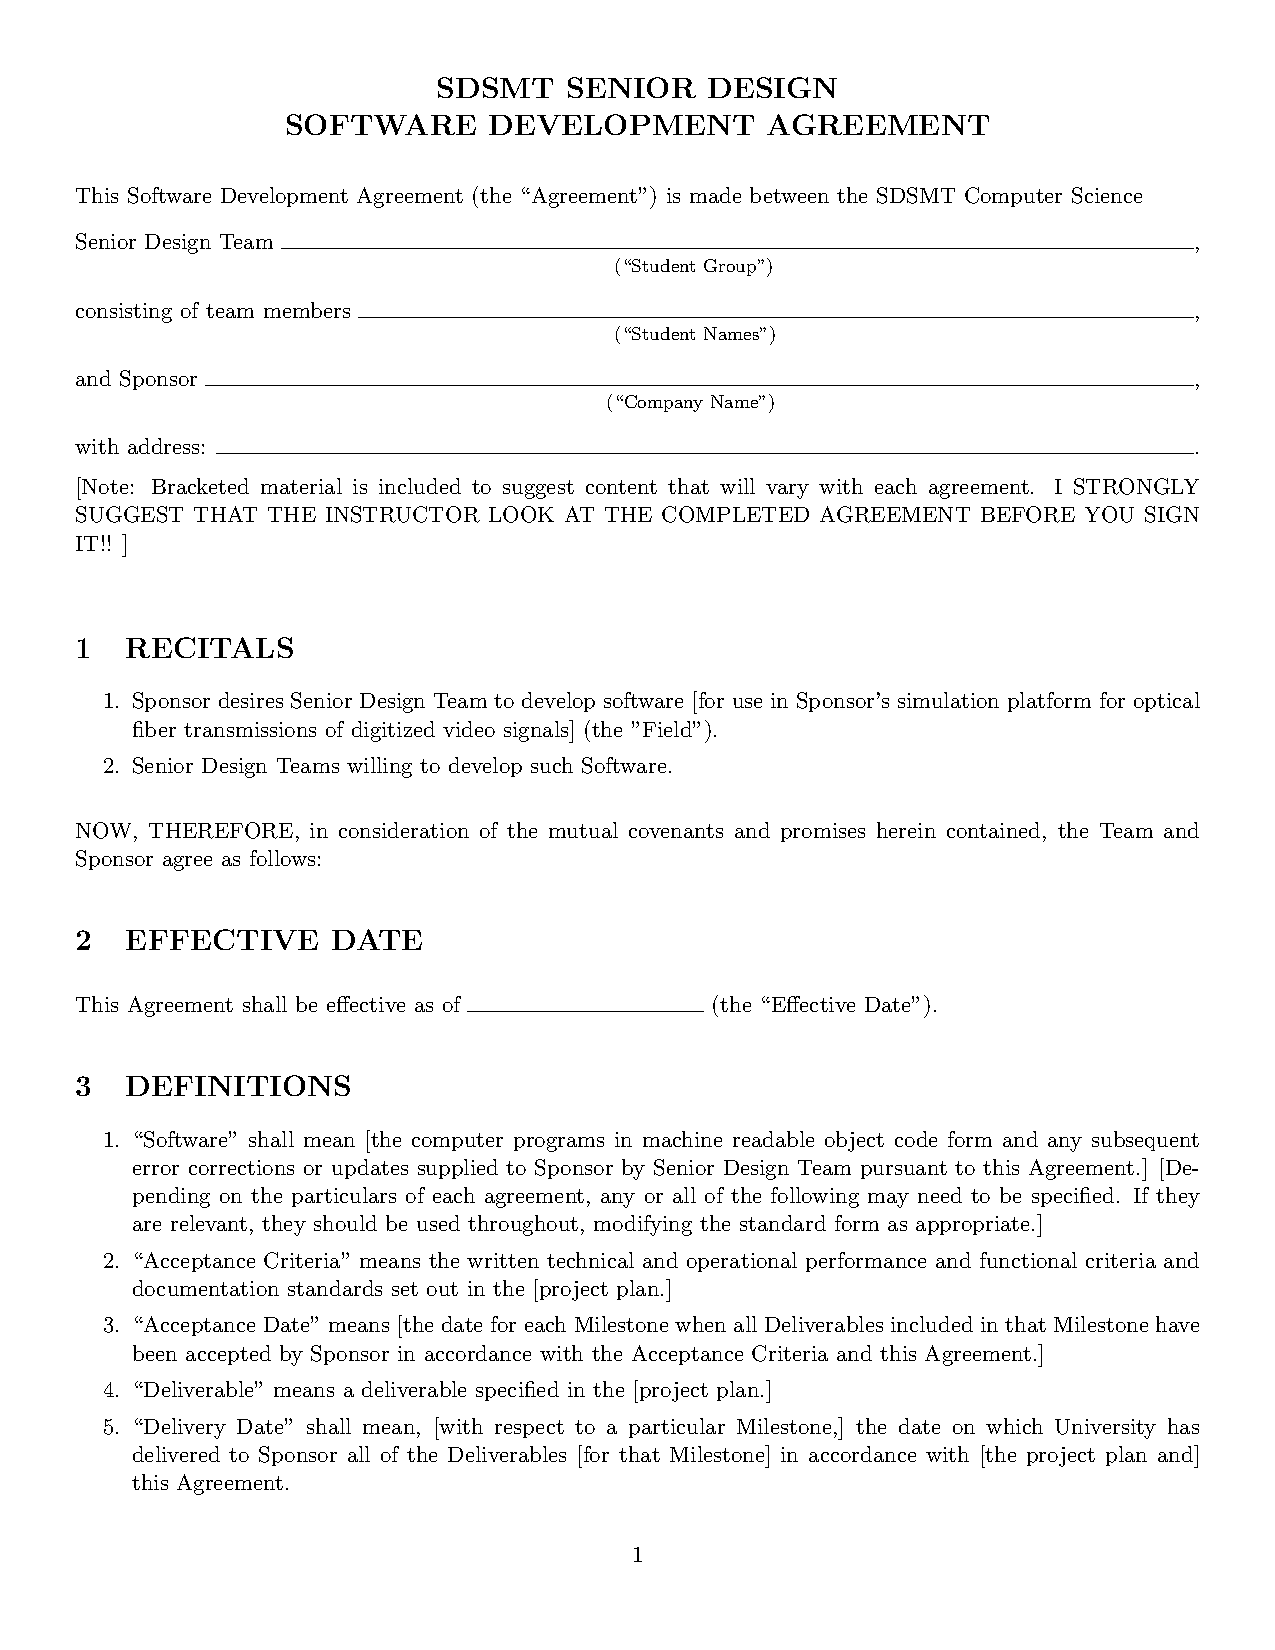
\includepdf[pages={1-4}]{SoftwareContract.pdf}
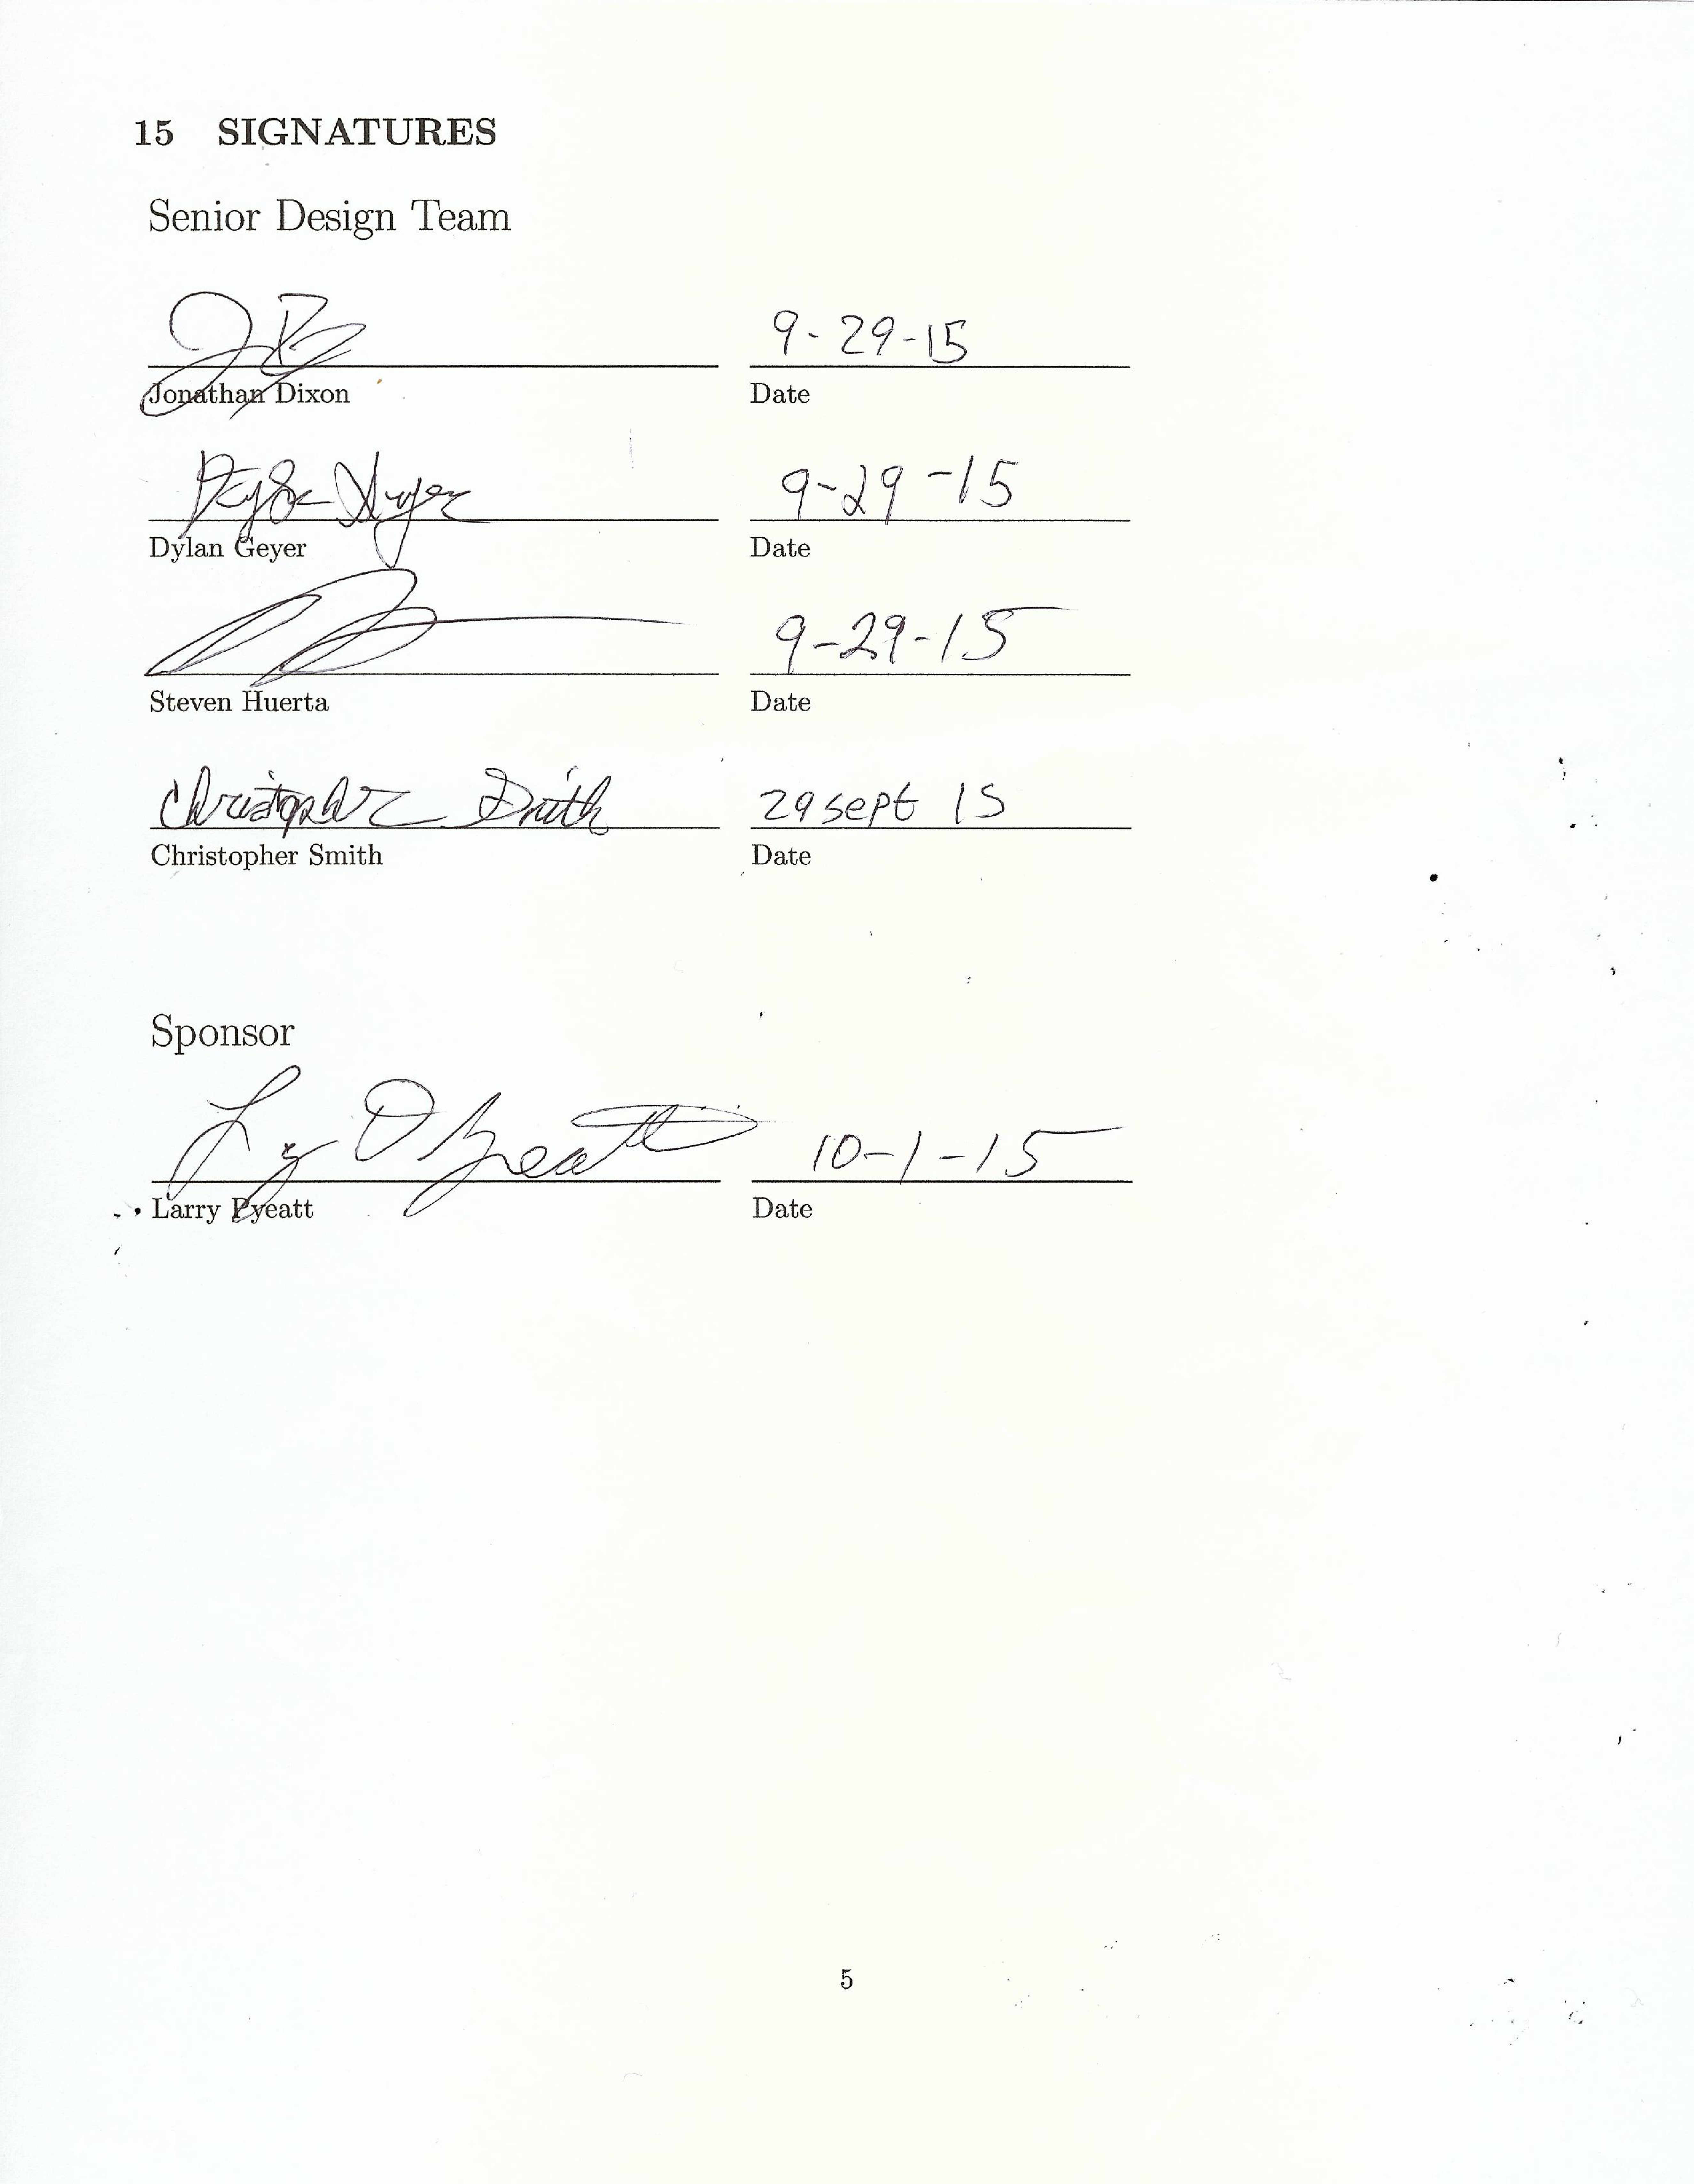
\includepdf[pages={1}]{sig_page.pdf}

% In our style file, appendices are numbered with capital letters
\appendix

\chapter{Product Description}


Write a description of the product to be developed.
Use sectioning commands as neccessary.
\vspace{2\baselineskip}

\centerline{\Large {\bf NOTE:} {\em This is part of the contract.}}



\chapter{Publications}   %% Research track 
% !TEX root = DesignDocument.tex


Research Track:  
This chapter will include any publications generated from the research.  Most likely these will be preprints and one will just include the pdf.

%\includepdf[pages={1-5}]{Pub1.pdf}



\chapter{Sprint Reports}
%!TEX root = DesignDocument.tex

\section{Sprint Report \#1}
% !TEX root = sprints.tex


\LARGE{\textbf{Team Overview}}
\\[-3mm]\noindent\makebox[\linewidth]{\rule{\textwidth}{0.4pt}}
\\[3mm]
\Large{\textbf{Name}}
\\ Expeditus 
\\[3mm]
\Large{\textbf{Members}}
\\ Jonathan Dixon, Dylan Geyer, Steven Huerta, Christopher Smith
\\[3mm]



\newpage
\section{Sprint Report \#2}
% !TEX root = sprints.tex
\noindent \Large{\textbf{Summary}}\\
\normalsize Team Expeditus was able to adapt to setbacks, and make progress on other tasks and goals of the project. Specifically, the team was able to make progress on the landing software, as well as find and implement a visual simulation that models the Pixhawk flight controller. The team was also able to coordinate with our advisor and school faculty for funding and ordering of our UAV platform and components. The restructuring of tasks for Sprint 2, does have a knock-on effect for Sprint 3. Sprint 3 will focus heavily on the building and testing of the UAV and its off-the-shelf components. Additionally, our client/advisor has suggested a different AI approach than the Artificial Neural Network(ANN). We will pursue this development during Sprint 3. Lastly, after meeting with the CENG/EE team several times, it was determined that while there is an opportunity for collaboration, time frames for both teams will not support collaboration.  Our team will continue, however, to work with the ME UGV team on the development of a landing pad functional for both teams.\\
\vspace{5mm}
\\
\noindent \Large{\textbf{Team Work}}
\normalsize
\begin{itemize}
\item \textbf{Julian Brackins:} Worked on tasks relating to Autonomous Landing.
\item \textbf{Jonathan Dixon:} Worked on tasks relating to Autonomous Landing.
\item \textbf{Dylan Geyer:} Worked on tasks relating to ordering parts for the UAV,
\item \textbf{Christopher Smith:} Worked on tasks relating to ordering parts for the UAV, as well as tasks relating to setting up a Simulation Environment.
\item \textbf{Steven Huerta:} Worked on tasks relating to ordering parts for the UAV, as well as tasks relating to setting up a Simulation Environment.
\end{itemize}

\vspace{5mm}
\noindent\Large{\textbf{Completed Backlog}}\\
\vspace{2mm}\\
\large{\textbf{Common Development Tasks}}
\normalsize
\begin{itemize}
\item \textbf{Setup Simulation Environment.}\\
The team now has a working software simulation of the Pixhawk 4, the flight controller for this build, that utilizes both ROS and Gazebo.
\item \textbf{Identify Parts Needed for UAV.} \\
The team was supplied with funding source. The team needed to additionally coordinate with the SDSMT UAV Team to order correct parts, as well as parts that would be useful to both groups to ensure redundancy in the event of component failure.
\item \textbf{Acquire parts needed for quadrotor} \\
Received approval for the ordering of the parts. Parts ordered. Expected delivery date of 11/9/15.
\end{itemize}

\vspace{3mm}
\noindent \large{\textbf{As a user, I want to communicate the waypoints to the UAV}}
\normalsize
\begin{itemize}
\item \textbf{Review code that communicates with quadrotor.}\\
 Software is available to access the flight controller through a GUI called APM Planner, available for Linux/Windows. Additionally, there is Mission Planner, available for Windows. Both will provide the ability of a user to communicate with the UAV.
\item \textbf{Review code that allows a user to input waypoints.}\\
Both APM Planner and Mission Planner allow the user to input waypoints through the GUI.  
\end{itemize}

\vspace{4mm}
\noindent \large{\textbf{As an owner, I want the UAV to autonomously take-off from the landing pad.}}
\normalsize
\begin{itemize}
\item \textbf{Review code that enables the quadrotor to autonomously take-off from landing pad.}\\
 This will be handled by Mission Planner/APM Planner.
\end{itemize}

\vspace{3mm}
\noindent \large{\textbf{As an owner, I want the UAV to autonomously navigate through a set of waypoints.}}
\normalsize
\begin{itemize}
\item \textbf{Review previous implementation for navigating waypoints.}\\
This will be handled by Mission Planner or APM Planner
\end{itemize}

\vspace{3mm}
\noindent \large{\textbf{As an owner, I want the UAV to autonomously return to the location of the landing pad.}} 
\normalsize
\begin{itemize}
\item \textbf{Review code that allows the autonomous return of the UAV to the landing pad.}\\
 This will be handled by Mission Planner or APM Planner. The built in autonomy will bring the UAV to a position near the landing pad, where either Visual Homography, Artificial Intelligence, or combination of the two will be responsible for landing the craft. It is estimated that the craft will be within 10 meters of the designated area. Discussions with UAV team members provide an estimate of 5 meters from their observations.
\end{itemize}

\vspace{3mm}
\noindent \large{\textbf{As an owner, I want the UAV to autonomously land on the landing pad without damaging the craft}}
\normalsize
\begin{itemize}
\item \textbf{Review previous implementation for autonomous landing.}\\
 The code was reviewed and is running. The software is correctly identifying the RGB lights and accurately reporting distance.
\end{itemize}

\vspace{3mm}
\noindent \large{\textbf{As an owner, I want the UAV to autonomously land on the landing pad with the correct orientation.}}
\normalsize
\begin{itemize}
\item \textbf{Review previous implementation for autonomous landing.}\\
 As reported above, the software is running and is able to detect the lights. This detection will allow the UAV to orient itself to align correctly with the landing pad.
\end{itemize}

\vspace{5mm}
\noindent\Large{\textbf{Uncompleted Tasks}}\\
\vspace{2mm}\\
\large{\textbf{Common Development Tasks}}
\normalsize
\begin{itemize}
\item \textbf{Build UAV}\\
 This will be completed during Sprint 3. Waiting for UAV parts to arrive.
\item \textbf{Test flight under manual control} \\
 Testing will be completed by Sprint 3. Waiting for UAV to be built.
\end{itemize}


\vspace{6mm}
\noindent\Large{\textbf{Prototype}}\\
\normalsize
There is a prototype document for Sprint 2 (found \href{https://github.com/SDSMT-CSC464-F15/landingpad/tree/master/Documents/Prototypes/Sprint_2}{here} in the repository), where this same material will be covered in much greater detail. This is only a brief description.
\begin{itemize}
\item \textbf{Visual Homography Code}\\
 The Visual Homography Code that was developed last year for the UAV Landing Project has been reviewed. The program successfully builds and much of it is likely to be reused towards providing the landing algorithm. The code can be found \href{https://github.com/SDSMT-CSC464-F15/landingpad/tree/master/2014-2015/led}{here} in the repository. The code requires that OpenCV has been installed. A cmake file is contained within the directory, so that after running cmake and make the program can be run by ./tracker. The tracker is looking for RGB blobs, so it may be better for testing to have some primary colors about to test. This program is currently providing correct distance in centimeters. 
\item \textbf{Simulation} \\
To test our landing algorithms in simulation, it would be very useful to have something that approximates the Pixhawk flight controller to communicate with for the purpose of supplying instructions to the controller, as well as receiving flight data. The PX4 development team have provided both Software-In-The-Loop and Hardware-In-The-Loop simulation environments. This will require Linux 14.04, ROS Distro Indigo or Jade, and the installation of a few repositories. These are detailed well in the setup document provided by the group \href{https://pixhawk.org/dev/ros/sitl#px4_ros_sitl_setup}{here}. However, \textbf{catkin\_ make} command did not build the meta-package correctly, as detailed in the instructions. Rather, \textbf{catkin build} will build the meta-package properly and the simulation will run with the assistance of an XBox controller (PS controllers will not work).
 \item \textbf{Ordering Parts} \\
 Over the course of Sprint 2, the team met with our advisor and faculty for purpose of receiving funding to create a new UAV platform for this project. The team also met with members of the UAV team to receive assistance and guidance in purchasing hardware that would be compatible with UAV team hardware. In the event of a component not functioning, our team would be able to utilize a component from the UAV team. After building a parts list for a hexrotor, we received approval from faculty for our purchase. A complete order list will be detailed in the Prototype document.
\end{itemize}

\newpage
\section{Sprint Report \#3}
% !TEX root = sprints.tex
\noindent \Large{\textbf{Summary}}\\
\normalsize Team Expeditus was unable to meet the expectations that it set for the conclusion of the first phase, ending with the conclusion of the third sprint. The team began this Sprint adapting to delays in receiving and testing UAV. The final contruction of the UAV was delayed beyond the end of this sprint due to ordering issues. Although the team had made progress on UAV construction, Simulation, and Landing approaches, the team acknowledges that we are currently behind schedule for Phase II. Workdays will be scheduled for team members to make up lost ground before the beginning of Sprint 4.\\
\vspace{5mm}
\\
\noindent \Large{\textbf{Team Work}}
\normalsize
\begin{itemize}
\item \textbf{Julian Brackins:} Worked on tasks relating to Autonomous Landing.
\item \textbf{Jonathan Dixon:} Worked on tasks relating to Autonomous Landing.
\item \textbf{Dylan Geyer:} Worked on tasks relating to assembly of UAV
\item \textbf{Christopher Smith:} Worked on tasks relating to setting up simulation environment and artificial intelligence landing approach.
\item \textbf{Steven Huerta:} Worked on tasks relating to setting up simulation environment and artificial intelligence landing approach.
\end{itemize}

\vspace{5mm}
\noindent\Large{\textbf{Completed Backlog}}\\
\vspace{2mm}\\
\large{\textbf{Common Development Tasks}}
\normalsize
\begin{itemize}
\item \textbf{Setup Simulation Environment.}\\
Software simulation of Pixhawk and Ardupilot (both make use of Mavlink which will be the handle used by our team to send commands and receive information from the flight controller). Simulations are successful in setup, however issues with communicating with Software-in-the-loop simulations.
\begin{itemize}
\item Pixhawk simulation (Pix4 ROS SITL): is working. The simulation will successfully emulate the flight controller and set up a simulation in Gazebo using ROS framework. Unable to send instructions to flight controller. Can successfully control UAV with Joystick to provide manual commands. Attempted to setup ground control station software (QGroundControl) to connect to Pixhawk SITL simulation. Unsuccessful in attempts to relay waypoint missions or arm the simulated UAV.
\item Arducopter (Ardupilot SITL with simulated Quadrotor): This simulation is working and the UAV can be controlled with a controller. Unable to communicate missions or controls via Mavlink API. A ROS waypoint publisher was developed to supply the simulation with commands to navigate to designated waypoints via MavROS(ROS wrapper for Mavlink). The publisher is successful in reaching the simulated ardu, however, the simulated UAV is unresponsive to ARM attempts, as well as commands to take-off or to navigate to waypoints.
\end{itemize}
Team members are hopeful that using the actual flight controller integration will be much smoother, as networking issues specific to simulated hardware are no longer a possible culprit, limiting the scope of troubleshooting.\\
\item \textbf{Acquire parts needed for quadrotor} \\
Frame, motors, and ESCs were received by Nov 13th. Waiting for remainder of order, including Flight Controller, GPS, power distribution board, and battery connector.
\item \textbf{Build UAV} \\
Construction began on the UAV. UAV frame is assembled. Motors and ESCs are attached. 
\end{itemize}

\vspace{3mm}
\noindent \large{\textbf{As an owner, I want the UAV to autonomously land on the landing pad without damaging the craft}}
\normalsize
\begin{itemize}
\item \textbf{Modify/Rewrite implementation as necessary}\\
The current setup of three points was found to insufficient to calculate the necessary transformation to unwarp the image. Team members have implemented a method to use a square, rather than a triangle.  
\end{itemize}

\vspace{3mm}
\noindent \large{\textbf{As an owner, I want the UAV to autonomously land on the landing pad with the correct orientation.}}
\normalsize
\begin{itemize}
\item \textbf{Modify/Rewrite implementation as necessary}\\
Changing the number of points from three to four causes some additional problem-solving. With three points, each can easily be assigned a color for clear distinction between points (Red, Green, Blue). The addition of a fourth causes some solving, as before only each of the RGB was used. Testing on simulated images, team members used Black. However, it is acknowledged that this will not be an available color. Once the color problem is solved, orientation will be regained.
\end{itemize}

\vspace{5mm}
\noindent\Large{\textbf{Uncompleted Tasks}}\\
\vspace{4mm}
\noindent \large{\textbf{As a user, I want to communicate the waypoints to the UAV}}
\normalsize
\begin{itemize}
\item \textbf{Modify/Rewrite imlementation as necessary}
\begin{itemize}
\item Waypoint Publisher: This is a test implementation to take a file of waypoints generated by a ground control station(GCS) and sequentially read them to supply the simulated flight controller with commands. This publisher is implemented with ROS, which will be the ultimate form of our landing command framework. The publisher is successful in sending messages, however, the UAV is not acting on the messages being passed. More troubleshooting will be needed.
\item Ground Control Station(GCS): There are some great GUI GCSs available. We have attempted to use QGroundControl to connect to the simulated flight controlled. This GCS is suggested by the developers of the flight controller simulations. 
\end{itemize} 
\end{itemize}

\vspace{3mm}
\noindent \large{\textbf{As an owner, I want the UAV to autonomously take-off from the landing pad.}}
\normalsize
\begin{itemize}
\item \textbf{Modify/Rewrite implementation as necessary}\\
This is dependent on successful communication using Mavlink/MavROS. Once the communication problem has been solved, the team will be able to use the GCS to provide the command to take-off. Additional support will not be needed (ie, no need to code custom interface).
\end{itemize}

\vspace{3mm}
\noindent \large{\textbf{As an owner, I want the UAV to autonomously navigate through a set of waypoints.}}
\normalsize
\begin{itemize}
\item \textbf{Modify/Rewrite implementation as necessary}\\
This is dependent on successful communication using Mavlink/MavROS. Once the communication problem has been solved, the team will be able to use the GCS to provide the command to navigation. Additional support will not be needed.
\end{itemize}


\vspace{3mm}
\noindent \large{\textbf{As an owner, I want the UAV to autonomously return to the location of the landing pad.}}
\normalsize
\begin{itemize}
\item \textbf{Modify/Rewrite implementation as necessary}\\
This is dependent on successful communication using Mavlink/MavROS. Once the communication problem has been solved, the team will be able to use the GCS to provide the command to navigate back to the landing pad. Additional support will not be needed.
\end{itemize}

\vspace{3mm}
\noindent \large{\textbf{As an owner, I want the UAV to autonomously land on the landing pad without damaging the craft}}
\normalsize
\begin{itemize}
\item \textbf{Propose AI Landing Algorithm}\\
Team members have discussed approaches, but were unable to dedicate a sufficient amount of time to create or begin an initial prototype.
\end{itemize}

\vspace{6mm}
\noindent\Large{\textbf{Prototype}}\\
\normalsize
There is a prototype document for Sprint 3 (found \href{https://github.com/SDSMT-CSC464-F15/landingpad/tree/master/Documents/Prototypes/Sprint_3}{here} in the repository), where this same material will be covered in much greater detail. This is only a brief description.
\begin{itemize}
\item \textbf{SIMULATION: \href{https://github.com/SDSMT-CSC464-F15/landingpad/blob/master/Documents/Prototypes/Sprint_3/ardusitl.pdf}{Ardu SITL}}\\
Software in the loop (SITL) was attempted again with many different simulators that work with ROS. One of them implemented there on version of a Mavlink and ROS interface and was not well documented on how to send commands besides direct motor. Another used Mavros and Mavlink for direct communication with the Pixhawk. However, it gave errors of invalid flight control unit and files did not hash properly so believed it was recieving invalid waypoint files that were generated by the mission planner. Hardware in the loop (HITL) was also attempted using the ardupilot with many different simulators. The same errors were also received with the file checksum integrety (MD5) and bot the SITL and HITL gave the same errors with all commands sent. Pixhawk was not attempted since it was received the week after the sprint, but will be attempted over break.
\item \textbf{SIMULATION: \href{https://github.com/SDSMT-CSC464-F15/landingpad/blob/master/Documents/Prototypes/Sprint_3/rossitl.pdf}{Pix ROS SITL Setup}}\\
These are the instructions for setting up the ROS SITL simulation. This simulation has the advantage of completely modelling the Pixhawk flight controller, the FCU that will be used by the team. The simulation will start an instance of Gazebo where a representation of a UAV controlled by the FCU is implemented. The UAV may be manually flown by the use of a joystick (XBox controller needed). 
\item \textbf{SIMULATION: \href{https://github.com/SDSMT-CSC464-F15/landingpad/blob/master/Documents/Prototypes/Sprint_3/gcsinstall.pdf}{QGroundControl Setup}} \\
These are the instructions for setting up the QGroundControl ground control station software for Ubuntu 14.04. QGroundControl provides a GUI that can link to the UAV's flight controller unit and supply missions such as autonomous take-off, waypoint navigation, and landing.  
\item \textbf{LANDING: \href{https://github.com/SDSMT-CSC464-F15/landingpad/blob/master/Documents/Prototypes/Sprint_3/CV_Sprint_3.pdf}{Visual Homography}}\\
This document discusses the current direction of Visual Landing approach. 
\item \textbf{UAV BUILD: \href{https://github.com/SDSMT-CSC464-F15/landingpad/blob/master/Documents/Prototypes/Sprint_3/BuildProcedure/BuildProcess.pdf}{Initial UAV Build}} \\
This document details the initial build of the UAV with current parts available.
\end{itemize}

\newpage
\section{Sprint Report \#4}
% !TEX root = sprints.tex
\noindent \Large{\textbf{Summary}}\\
\normalsize Team Expeditus was able to accomplish most of the objectives for sprint 3.5 and 4. Sprint 3.5 focused mostly on designing a new base plate for the hexrotor and calibrating the flight controller. During this sprint it was agreed on by the team members to set aside work on the simulation as too much time was being consumed by issues encountered. The UAV was able to flown under manual control successfully by the end of Sprint 3.5. Sprint 4 focused on autonomous flight testing, flight control specific message passing in the ROS framework, and reapproach to vision. By the end of the sprint the autonomous flight was successfully tested and a software package for AR tag tracking was successfully compiled and run.\\
\vspace{5mm}
\\
\noindent \Large{\textbf{Team Work}}
\normalsize
\begin{itemize}
\item \textbf{Jonathan Dixon:} Worked on UAV build, AR tracking, and UAV flight.
\item \textbf{Dylan Geyer:} Worked on UAV build, AR tracking, and UAV flight.
\item \textbf{Christopher Smith:} Worked on UAV build, message passing, AR tracking, and UAV flight. 
\item \textbf{Steven Huerta:} Worked on UAV build, AR tracking, and UAV flight. 
\end{itemize}

\vspace{5mm}
\noindent\Large{\textbf{Completed Backlog}}\\
\vspace{2mm}\\
\large{\textbf{Common Development Tasks}}
\normalsize
\begin{itemize}
\item \textbf{Build UAV.}\\
The UAV was assembled before winter break, however, it was apparent that the power distribution board did not fit appropriately, and in addition, the team realized that more room would be needed on the center plate to accomodate the control hardware and sensors. Team members modeled a new plate that was larger and printed the plates. These printed plates will be temporary, as carbon fiber will be used for the final build. The new plates provided the necessary room from the distro board, as well as being able to easily accomodate the flight controller, Odroid, and other sensors.\\
\item \textbf{Test flight under manual control} \\
The UAV was first tested under manual control within the King Center at SDSMT. The manual flight was successful and validated the build. The UAV was responsive to pilot controls.
\item \textbf{Autonomous Flight} \\
The testing of the autonomous flight validated the capability of the flight controller to provide the hexrotor speed controllers the necessary and correct signals, as well as validating the build of the UAV.

This objective is also relevant to the following user stories:
\begin{itemize}
\item \textbf{U-1 As a user, I want to communicate the waypoints to the UAV:} \\
The team successfully sent a series of "missions" to the flight controller including take-off, waypoint navigation goals, and landing. The team used QGroundControl GUI to easily mark points and define the associated action for the UAV.
\item \textbf{O-1 As an owner, I want the UAV to autonomously take-off from the landing pad:} \\
The mission provided to the flight controller instructed the UAV to take-off and achieve a certain height before executing the next mission. The UAV repeatedly executed these instructions according to parameters provided throught the GUI mission setup.
\item \textbf{O-2 As an owner, I want the UAV to autonomously navigate through a set of waypoints:} \\
The UAV navigated to the waypoints assigned. This process was repeated for a set of waypoints to ensure that navigation of these points was being sucessfully handled by the flight controller. The team also observed that despite a flexible frame, caused by the material used in our temporary assembly plates, and some unsecured rotation in one of the rotor arms, the flight controller still successfully navigated through the waypoints.
\item \textbf{O-3 As an owner, I want the UAV to autonomously return to the location of the landing pad:} \\
The UAV navigated back to the location of the landing area designated. Though this was achieved simply by defining the return as the last waypoint mission that the flight controller will execute. It was also observed that if the user uses the landing mission, the flight controller will determine the direct line to land at that point, which is definitely problematic if the landing area is higher than the altitude of the UAV. It causes the UAV to "skip" along the surface. However, this will not be an issue for our team, as we will not be using the landing mission. \\
The navigation is very accurate relative to expectations. The same navigation points used for takeoff were used for the final point of navigation and landing. The flight controller consistently set UAV within two feet of the takeoff point. This has caused the team to re-evaluate the needs for a landing pad. The team feels confident that with the GPS, the flight controller will allow the UAV to navigate to a point where an AR tag alone can be used to provide visual guidance to the UAV.
\end{itemize} 
\end{itemize}


\vspace{5mm}
\noindent\Large{\textbf{Uncompleted Tasks}}\\
\vspace{4mm}
\noindent \large{\textbf{Common Development Tasks}}
\normalsize
\begin{itemize}
\item \textbf{Setup Hexrotor Simulation in Gazebo}
The team has decided to indefinitely postpone development of the specific hexrotor simulation. The time invested on resolving software and hardware conflicts was monopolizing project time.
\end{itemize} 

\vspace{3mm}
\noindent \large{\textbf{As an owner, I want the UAV to autonomously land on the landing pad without damaging the craft}}
\normalsize
\begin{itemize}
\item \textbf{Landing Algorithm Simulation}\\
As the team has ceased simulation development, initial testing for the landing algorithm will not occur using the simulation. The proposed method for testing is to review logs generated by our vision guided landing solution while passing the UAV, without props, over the landing AR tag and reviewing the messages passed to the flight controller for descent. The team will specifically test for a controlled landing that will prevent damage to the UAV or the landing pad from the force of impact.
\item \textbf{Modify/Rewrite implementation as necessary}\\
Though not completed, progress was made on modifying our implementation of the landing algorithm to only include the AR tag tracking. The tracking tool that we have successfully tested will provide us with distance information necessary to correctly judge the distance from our landing target, as well as calculate a safe rate of descent.
\end{itemize}



\vspace{3mm}
\noindent \large{\textbf{As an owner, I want the UAV to autonomously land on the landing pad with the correct orientation.}}
\normalsize
\begin{itemize}
\item \textbf{Landing Algorithm Simulation}\\
As mentioned previously, as our simulation development has ended, our team will utilize the sensors to generate log data to evaluate. The team will specifically test for orientation corrections that will provide the correct alignment on landing.
\item \textbf{Modify/Rewrite implementation as necessary}\\
As mentioned previously, our visual landing approach has changed. We hope to be able to easily modify the existing software to provide information regarding the orientation of the AR tag to use to change the orientation of the UAV as necessary during landing.
\end{itemize}

\vspace{6mm}
\noindent\Large{\textbf{Prototype}}\\
\normalsize
Still Need to create some descriptions for the prototype and descriptions


\newpage
\section{Sprint Report \#5}
% !TEX root = sprints.tex
\noindent \Large{\textbf{Summary}}\\
\normalsize Team Expeditus was unfortunately unable to complete the tasks for sprint 5, but the team was able to make measurable progress towards the goals. After deciding not to pursue simulation, the team members began to focus on message passing and offboard control between the flight controller and the Odroid. After multiple issues with multiple approaches to the AR tag tracking, the team was able to successfully get the AR Track Alvar library up and running.
\vspace{5mm}
\\
\noindent \Large{\textbf{Team Work}}
\normalsize
\begin{itemize}
\item \textbf{Jonathan Dixon:} Worked AR tracking.
\item \textbf{Dylan Geyer:} Worked on AR tracking.
\item \textbf{Christopher Smith:} Worked on message passing and offboard control. 
\item \textbf{Steven Huerta:} Worked on AR tracking. 
\end{itemize}

\vspace{5mm}
\noindent\Large{\textbf{Uncompleted Tasks}}\\
\vspace{2mm}\\
\noindent \large{\textbf{As an owner, I want the UAV to autonomously land on the landing pad without damaging the craft}}
\normalsize
\begin{itemize}
\item \textbf{Setup Hexrotor Simulation in Gazebo}
The team has decided to indefinitely postpone development of the specific hexrotor simulation. The time invested on resolving software and hardware conflicts was monopolizing project time.
\end{itemize} 

\vspace{3mm}
\noindent \large{\textbf{As an owner, I want the UAV to autonomously land on the landing pad without damaging the craft}}
\normalsize
\begin{itemize}
\item \textbf{Landing Algorithm Simulation}\\
As the team has ceased simulation development, initial testing for the landing algorithm will not occur using the simulation. The proposed method for testing is to review logs generated by our vision guided landing solution while passing the UAV, without props, over the landing AR tag and reviewing the messages passed to the flight controller for descent. The team will specifically test for a controlled landing that will prevent damage to the UAV or the landing pad from the force of impact.
\item \textbf{Modify/Rewrite implementation as necessary}\\
Though not completed, progress was made on modifying our implementation of the landing algorithm to only include the AR tag tracking. The tracking tool (fig.~\ref{fig:artracker}) that we have successfully tested will provide us with distance information necessary to correctly judge the distance from our landing target, as well as calculate a safe rate of descent.
\begin{figure}[h]
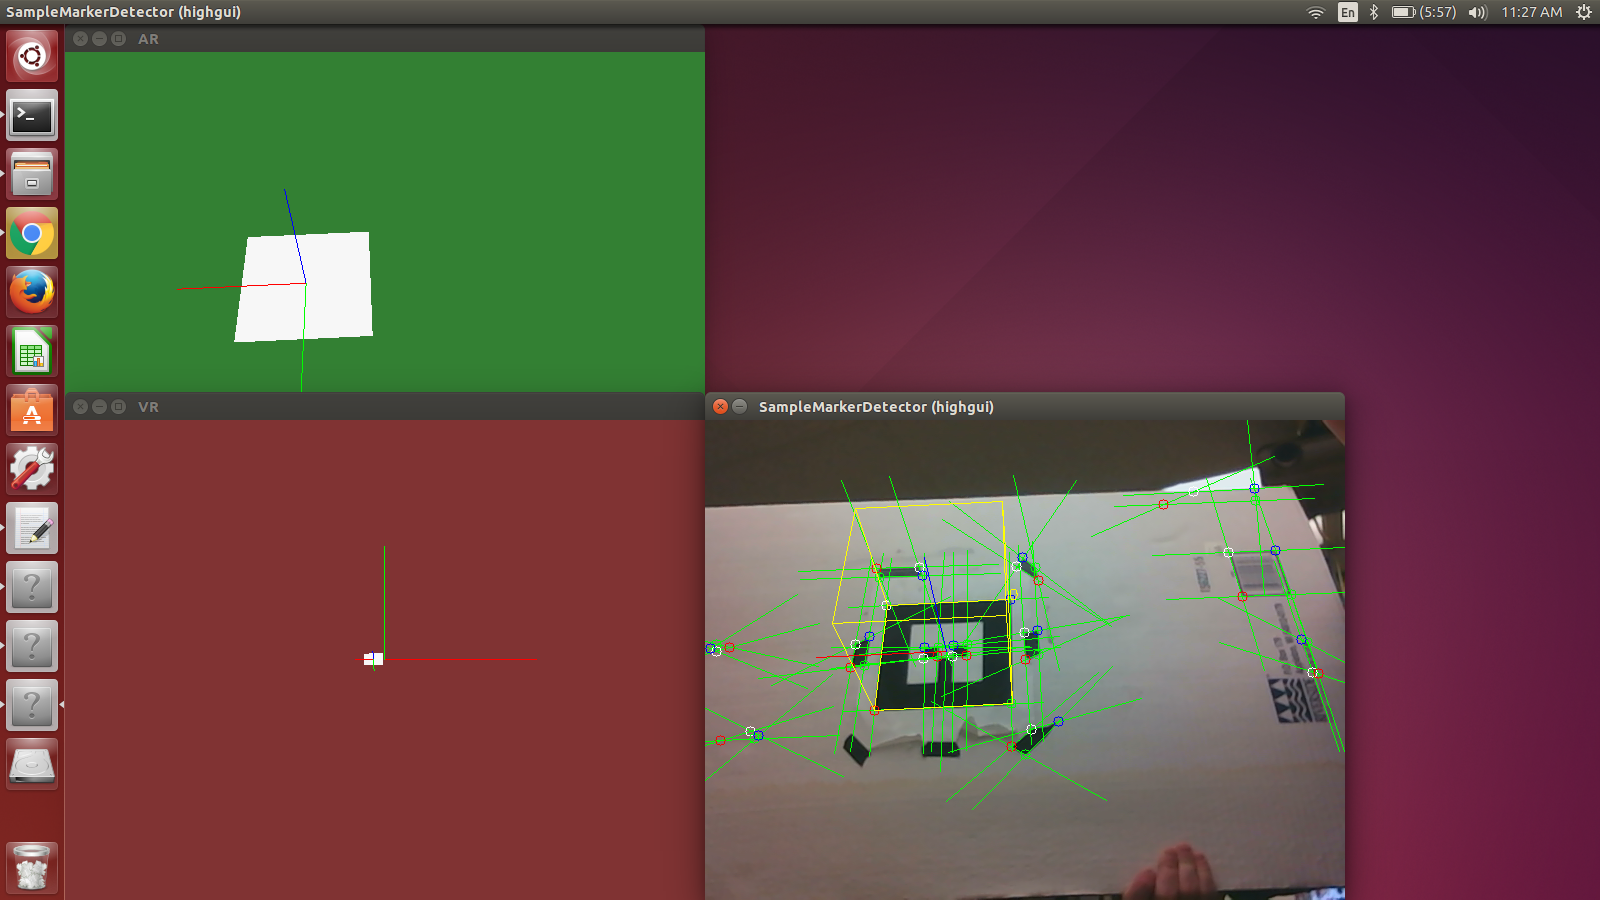
\includegraphics[width=8cm]{AlvarExample.png}
\centering
\caption{ALVAR AR Tracker testing with laptop webcam}
\label{fig:artracker}
\end{figure}

\end{itemize}


\vspace{3mm}
\noindent \large{\textbf{As an owner, I want the UAV to autonomously land on the landing pad with the correct orientation.}}
\normalsize
\begin{itemize}
\item \textbf{Landing Algorithm Simulation}\\
As mentioned previously, as our simulation development has ended, our team will utilize the sensors to generate log data to evaluate. The team will specifically test for orientation corrections that will provide the correct alignment on landing.
\item \textbf{Modify/Rewrite implementation as necessary}\\
As mentioned previously, our visual landing approach has changed. We hope to be able to easily modify the existing software to provide information regarding the orientation of the AR tag to use to change the orientation of the UAV as necessary during landing.
\end{itemize}

\vspace{6mm}
\noindent\Large{\textbf{Prototype}}\\
\normalsize
Our prototype for this sprint is mainly just an assembled hexrotor UAV that is able to follow GPS waypoints. Throughout the assembly process, we did small tests to be sure that we were on the right track. At first, we just kept the UAV in the lab and turned to rotors to verify that they were wired correctly and spinning in the right directions. We then had a manual test flight in the gym, where we discovered that the UAV is quite stable and responsive. Finally, we tested the GPS waypoint navigation with a series of flights. We started small, just having the UAV fly to the end of the driveway at first, eventually working our way up to having the UAV take off, move through a series of waypoints, and return to land on the same location it took off from. Over the course of our testing, we estimate that we will be able to trust the GPS to get us above our landing pad. As stated above, this means that we feel confident that we will be able to trust GPS to get us directly above the landing pad. \newline\newline
We have videos of these GPS tests up on \href{https://www.youtube.com/channel/UCfcuqDXKMLgbUWu3rt9rITA}{YouTube}.




\chapter{Industrial Experience and Resumes}
% !TEX root = SystemTemplate.tex


\section{Resumes}

Your resumes are included here.  See the source file (industrial.tex) and uncomment the PDF includes to see how this works.  If your resume is written in \LaTeX\ then you can just insert the \LaTeX\ source code.

%    \includepdf[pages={1}]{report.pdf}  %% example of limited page include

%     \includepdf{resume1.pdf}
%     \includepdf{resume2.pdf}
%     \includepdf{resume3.pdf}

\section{ABET:  Industrial Experience Reports}

\subsection{Name1}

% \includepdf{name1.pdf}

\subsection{Name2}

% \includepdf{name2.pdf}

\subsection{Name3}

% \includepdf{name3.pdf}




\chapter{Acknowledgment}
\label{SpecialThanks}  
Thanks  

\chapter{Supporting Materials}

This document will contain several appendices used as a way to separate out major 
component details, logic details, or tables of information.  Use of this structure 
will help keep the document clean, readable, and organized. 



% chapters in backmatter don't have numbers, but they appear in the
% table of contents, and are numbered BM-X where X is the page number
% relative to where the backmatter begins.
\backmatter

%% Example
%\chapter{Course Syllabus}
%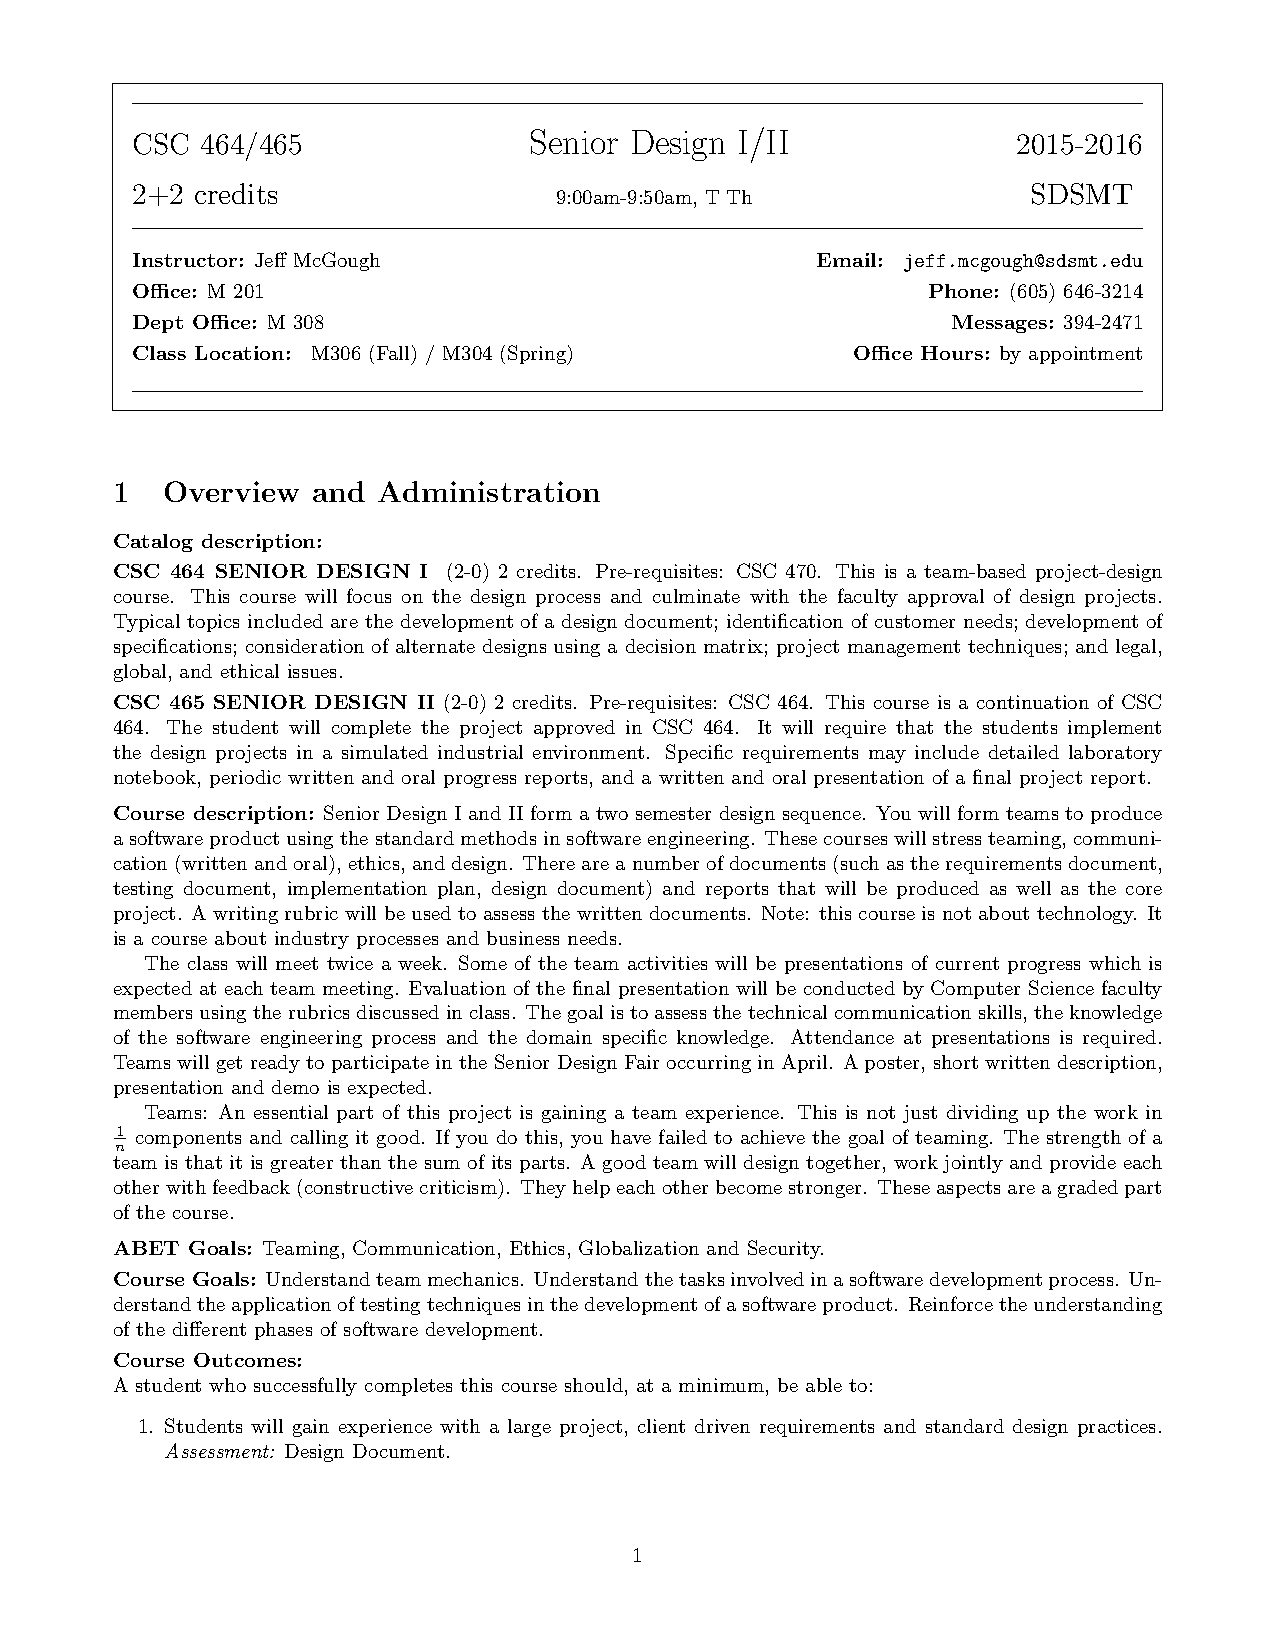
\includepdf[pages={1-17}]{syllabus.pdf}

%%% Remove after reading
\chapter{\LaTeX\ Example}
% !TEX root = SystemTemplate.tex


\LaTeX\xspace sample file:  {\color{red} Remove from submitted materials}

\section{Introduction}
This is a sample input file.  Comparing it with the output it
generates can show you how to produce a simple document of
your own.

\section{Ordinary Text}  % Produces section heading.  Lower-level
                                    % sections are begun with similar 
                                    % \subsection and \subsubsection commands.

The ends  of words and sentences are marked 
  by   spaces. It  doesn't matter how many 
spaces    you type; one is as good as 100.  The
end of   a line counts as a space.

One   or more   blank lines denote the  end 
of  a paragraph.  

Since any number of consecutive spaces are treated like a single
one, the formatting of the input file makes no difference to
      \TeX,         % The \TeX command generates the TeX logo.
but it makes a difference to you.  
When you use
      \LaTeX,       % The \LaTeX command generates the LaTeX logo.
making your input file as easy to read as possible
will be a great help as you write your document and when you
change it.  This sample file shows how you can add comments to
your own input file.

Because printing is different from typewriting, there are a 
number of things that you have to do differently when preparing 
an input file than if you were just typing the document directly.  
Quotation marks like 
       ``this'' 
have to be handled specially, as do quotes within quotes: 
       ``\,`this'                  % \, separates the double and single quote.
        is what I just 
        wrote, not  `that'\,''.  

Dashes come in three sizes: an 
       intra-word 
dash, a medium dash for number ranges like 
       1--2, 
and a punctuation 
       dash---like 
this.

A sentence-ending space should be larger than the space between words
within a sentence.  You sometimes have to type special commands in
conjunction with punctuation characters to get this right, as in the
following sentence.
       Gnats, gnus, etc.\    % `\ ' makes an inter-word space.
       all begin with G\@.   % \@ marks end-of-sentence punctuation.
You should check the spaces after periods when reading your output to
make sure you haven't forgotten any special cases.
Generating an ellipsis 
       \ldots\    % `\ ' needed because TeX ignores spaces after 
                  % command names like \ldots made from \ + letters.
                  %
                  % Note how a `%' character causes TeX to ignore the 
                  % end of the input line, so these blank lines do not
                  % start a new paragraph.
with the right spacing around the periods 
requires a special  command.  

\TeX\ interprets some common characters as commands, so you must type
special commands to generate them.  These characters include the
following: 
       \$ \& \% \# \{ and \}.

In printing, text is emphasized by using an
       {\em italic\/}  % The \/ command produces the tiny extra space that
                       % should be added between a slanted and a following
                       % unslanted letter.
type style.  

\begin{em}
   A long segment of text can also be emphasized in this way.  Text within
   such a segment given additional emphasis 
          with\/ {\em Roman} 
   type.  Italic type loses its ability to emphasize and become simply
   distracting when used excessively.  
\end{em}

It is sometimes necessary to prevent \TeX\ from breaking a line where
it might otherwise do so.  This may be at a space, as between the
``Mr.'' and ``Jones'' in
       ``Mr.~Jones'',        % ~ produces an unbreakable interword space.
or within a word---especially when the word is a symbol like
       \mbox{\em itemnum\/} 
that makes little sense when hyphenated across 
       lines.

Footnotes\footnote{This is an example of a footnote.}
pose no problem.

\TeX\ is good at typesetting mathematical formulas like
       \( x-3y = 7 \) 
or
       \( a_{1} > x^{2n} / y^{2n} > x' \).
Remember that a letter like
       $x$        % $ ... $  and  \( ... \)  are equivalent
is a formula when it denotes a mathematical symbol, and should
be treated as one.

\section{Displayed Text}

Text is displayed by indenting it from the left margin.
Quotations are commonly displayed.  There are short quotations
\begin{quote}
   This is a short a quotation.  It consists of a 
   single paragraph of text.  There is no paragraph
   indentation.
\end{quote}
and longer ones.
\begin{quotation}
   This is a longer quotation.  It consists of two paragraphs
   of text.  The beginning of each paragraph is indicated
   by an extra indentation.

   This is the second paragraph of the quotation.  It is just
   as dull as the first paragraph.
\end{quotation}
Another frequently-displayed structure is a list.
The following is an example of an {\em itemized} list.
\begin{itemize}
   \item  This is the first item of an itemized list.  Each item 
          in the list is marked with a ``tick''.  The document
          style determines what kind of tick mark is used.

   \item  This is the second item of the list.  It contains another
          list nested inside it.  The inner list is an {\em enumerated}
          list.
          \begin{enumerate}
              \item This is the first item of an enumerated list that
                    is nested within the itemized list.

              \item This is the second item of the inner list.  \LaTeX\
                    allows you to nest lists deeper than you really should.
          \end{enumerate}
          This is the rest of the second item of the outer list.  It
          is no more interesting than any other part of the item.
   \item  This is the third item of the list.
\end{itemize}
You can even display poetry.
\begin{verse}
   There is an environment for verse \\    % The \\ command separates lines
   Whose features some poets will curse.   % within a stanza.

                           % One or more blank lines separate stanzas.

   For instead of making\\
   Them do {\em all\/} line breaking, \\
   It allows them to put too many words on a line when they'd 
   rather be forced to be terse.
\end{verse}

Mathematical formulas may also be displayed.  A displayed formula is
one-line long; multi-line formulas require special formatting
instructions.
   \[  x' + y^{2} = z_{i}^{2}\]
Don't start a paragraph with a displayed equation, nor make
one a paragraph by itself.

\section{Build process}

To build \LaTeX\ documents you need the latex program.  It is free and available on all operating systems.   Download and install.  Many of us use the TexLive distribution and are very happy with it.    You can use a editor and command line or use an IDE.  To build this document via command line:

\begin{verbatim}
alta>  pdflatex SystemTemplate
\end{verbatim}
If you change the bib entries, then you need to update the bib files:
\begin{verbatim}
alta>  pdflatex SystemTemplate
alta>  bibtex SystemTemplate
alta>  pdflatex SystemTemplate
alta>  pdflatex SystemTemplate
\end{verbatim}

The template files provided also contain a Makefile, which will
make things much easier.  

\section*{Acknowledgment}
Thanks to Leslie Lamport.  






\end{document}
